\documentclass[a4paper,11pt,oneside]{memoir}

% Castellano
\usepackage[spanish]{babel}
\selectlanguage{spanish}
\usepackage[utf8x]{inputenc} 
\usepackage{placeins}
\usepackage{eurosym} % para el euro

\RequirePackage{booktabs}
\RequirePackage[table]{xcolor}
\RequirePackage{xtab}
\RequirePackage{multirow}

% Links
\usepackage[colorlinks]{hyperref}
\hypersetup{
	allcolors = {red}
}

% Ecuaciones
\usepackage{amsmath}

% Rutas de fichero / paquete
\newcommand{\ruta}[1]{{\sffamily #1}}

% Párrafos
\nonzeroparskip


% Imagenes
\usepackage{graphicx}
\newcommand{\imagen}[2]{
	\begin{figure}[!h]
		\centering
		\includegraphics[width=0.9\textwidth]{#1}
		\caption{#2}\label{fig:#1}
	\end{figure}
	\FloatBarrier
}

\newcommand{\imagenflotante}[2]{
	\begin{figure}%[!h]
		\centering
		\includegraphics[width=0.9\textwidth]{#1}
		\caption{#2}\label{fig:#1}
	\end{figure}
}



% El comando \figura nos permite insertar figuras comodamente, y utilizando
% siempre el mismo formato. Los parametros son:
% 1 -> Porcentaje del ancho de página que ocupará la figura (de 0 a 1)
% 2 --> Fichero de la imagen
% 3 --> Texto a pie de imagen
% 4 --> Etiqueta (label) para referencias
% 5 --> Opciones que queramos pasarle al \includegraphics
% 6 --> Opciones de posicionamiento a pasarle a \begin{figure}
\newcommand{\figuraConPosicion}[6]{%
  \setlength{\anchoFloat}{#1\textwidth}%
  \addtolength{\anchoFloat}{-4\fboxsep}%
  \setlength{\anchoFigura}{\anchoFloat}%
  \begin{figure}[#6]
    \begin{center}%
      \Ovalbox{%
        \begin{minipage}{\anchoFloat}%
          \begin{center}%
            \includegraphics[width=\anchoFigura,#5]{#2}%
            \caption{#3}%
            \label{#4}%
          \end{center}%
        \end{minipage}
      }%
    \end{center}%
  \end{figure}%
}

%
% Comando para incluir imágenes en formato apaisado (sin marco).
\newcommand{\figuraApaisadaSinMarco}[5]{%
  \begin{figure}%
    \begin{center}%
    \includegraphics[angle=90,height=#1\textheight,#5]{#2}%
    \caption{#3}%
    \label{#4}%
    \end{center}%
  \end{figure}%
}
% Para las tablas
\newcommand{\otoprule}{\midrule [\heavyrulewidth]}
%
% Nuevo comando para tablas pequeñas (menos de una página).
\newcommand{\tablaSmall}[5]{%
 \begin{table}[htb]
  \begin{center}
   \rowcolors {2}{gray!35}{}
   \begin{tabular}{#2}
    \toprule
    #4
    \otoprule
    #5
    \bottomrule
   \end{tabular}
   \caption{#1}
   \label{tabla:#3}
  \end{center}
 \end{table}
}

%
% Nuevo comando para tablas pequeñas (menos de una página).
\newcommand{\tablaSmallSinColores}[5]{%
 \begin{table}[H]
  \begin{center}
   \begin{tabular}{#2}
    \toprule
    #4
    \otoprule
    #5
    \bottomrule
   \end{tabular}
   \caption{#1}
   \label{tabla:#3}
  \end{center}
 \end{table}
}

\newcommand{\tablaApaisadaSmall}[5]{%
\begin{landscape}
  \begin{table}
   \begin{center}
    \rowcolors {2}{gray!35}{}
    \begin{tabular}{#2}
     \toprule
     #4
     \otoprule
     #5
     \bottomrule
    \end{tabular}
    \caption{#1}
    \label{tabla:#3}
   \end{center}
  \end{table}
\end{landscape}
}

%
% Nuevo comando para tablas grandes con cabecera y filas alternas coloreadas en gris.
\newcommand{\tabla}[6]{%
  \begin{center}
    \tablefirsthead{
      \toprule
      #5
      \otoprule
    }
    \tablehead{
      \multicolumn{#3}{l}{\small\sl continúa desde la página anterior}\\
      \toprule
      #5
      \otoprule
    }
    \tabletail{
      \hline
      \multicolumn{#3}{r}{\small\sl continúa en la página siguiente}\\
    }
    \tablelasttail{
      \hline
    }
    \bottomcaption{#1}
    \rowcolors {2}{gray!35}{}
    \begin{xtabular}{#2}
      #6
      \bottomrule
    \end{xtabular}
    \label{tabla:#4}
  \end{center}
}

%
% Nuevo comando para tablas grandes con cabecera.
\newcommand{\tablaSinColores}[6]{%
  \begin{center}
    \tablefirsthead{
      \toprule
      #5
      \otoprule
    }
    \tablehead{
      \multicolumn{#3}{l}{\small\sl continúa desde la página anterior}\\
      \toprule
      #5
      \otoprule
    }
    \tabletail{
      \hline
      \multicolumn{#3}{r}{\small\sl continúa en la página siguiente}\\
    }
    \tablelasttail{
      \hline
    }
    \bottomcaption{#1}
    \begin{xtabular}{#2}
      #6
      \bottomrule
    \end{xtabular}
    \label{tabla:#4}
  \end{center}
}

%
% Nuevo comando para tablas grandes sin cabecera.
\newcommand{\tablaSinCabecera}[5]{%
  \begin{center}
    \tablefirsthead{
      \toprule
    }
    \tablehead{
      \multicolumn{#3}{l}{\small\sl continúa desde la página anterior}\\
      \hline
    }
    \tabletail{
      \hline
      \multicolumn{#3}{r}{\small\sl continúa en la página siguiente}\\
    }
    \tablelasttail{
      \hline
    }
    \bottomcaption{#1}
  \begin{xtabular}{#2}
    #5
   \bottomrule
  \end{xtabular}
  \label{tabla:#4}
  \end{center}
}



\definecolor{cgoLight}{HTML}{EEEEEE}
\definecolor{cgoExtralight}{HTML}{FFFFFF}

%
% Nuevo comando para tablas grandes sin cabecera.
\newcommand{\tablaSinCabeceraConBandas}[5]{%
  \begin{center}
    \tablefirsthead{
      \toprule
    }
    \tablehead{
      \multicolumn{#3}{l}{\small\sl continúa desde la página anterior}\\
      \hline
    }
    \tabletail{
      \hline
      \multicolumn{#3}{r}{\small\sl continúa en la página siguiente}\\
    }
    \tablelasttail{
      \hline
    }
    \bottomcaption{#1}
    \rowcolors[]{1}{cgoExtralight}{cgoLight}

  \begin{xtabular}{#2}
    #5
   \bottomrule
  \end{xtabular}
  \label{tabla:#4}
  \end{center}
}




\graphicspath{ {./img/} }

% Capítulos
\chapterstyle{bianchi}
\newcommand{\capitulo}[2]{
	\setcounter{chapter}{#1}
	\setcounter{section}{0}
	\chapter*{#2}
	\addcontentsline{toc}{chapter}{#2}
	\markboth{#2}{#2}
}

% Apéndices
\renewcommand{\appendixname}{Apéndice}
\renewcommand*\cftappendixname{\appendixname}

\newcommand{\apendice}[1]{
	%\renewcommand{\thechapter}{A}
	\chapter{#1}
}

\renewcommand*\cftappendixname{\appendixname\ }

% Formato de portada
\makeatletter
\usepackage{xcolor}
\newcommand{\tutor}[1]{\def\@tutor{#1}}
\newcommand{\course}[1]{\def\@course{#1}}
\definecolor{cpardoBox}{HTML}{E6E6FF}
\def\maketitle{
  \null
  \thispagestyle{empty}
  % Cabecera ----------------
\noindent
\includegraphics[width=\textwidth]{cabecera}\vspace{1cm}%
  \vfill
  % Título proyecto y escudo informática ----------------
  \colorbox{cpardoBox}{%
    \begin{minipage}{.8\textwidth}
      \vspace{.5cm}\Large
      \begin{center}
      \textbf{TFG del Grado en Ingeniería Informática}\vspace{.6cm}\\
      \textbf{\LARGE\@title{}}
      \end{center}
      \vspace{.2cm}
    \end{minipage}

  }%
  \hfill\begin{minipage}{.20\textwidth}
    
\includegraphics[width=\textwidth]{escudoInfor}
  \end{minipage}
  \vfill
  % Datos de alumno, curso y tutores ------------------
  \begin{center}%
  {%
    \noindent\LARGE
    Presentado por \@author{}\\ 
    en Universidad de Burgos --- \@date{}\\
    Tutor: \@tutor{}\\
  }%
  \end{center}%
  \null
  \cleardoublepage
  }
\makeatother


% Datos de portada
\title{título del TFG \\Documentación Técnica}
\author{nombre alumno}
\tutor{nombre tutor}
\date{\today}

\begin{document}

\maketitle



\cleardoublepage



%%%%%%%%%%%%%%%%%%%%%%%%%%%%%%%%%%%%%%%%%%%%%%%%%%%%%%%%%%%%%%%%%%%%%%%%%%%%%%%%%%%%%%%%



\frontmatter


\clearpage

% Indices
\tableofcontents

\clearpage

\listoffigures

\clearpage

%\listoftables

%\clearpage

\mainmatter

\appendix

\apendice{Manuales}

\section{Introducción}

\section{Planificación temporal}

A continuación se realiza una breve explicación de las tareas realizadas en cada iteración.

\subsection{Iteración 1 [28/10/2015 - 04/11/2015]}
Esta iteración dura una semana. En ella se realiza principalmente 3 tareas.
Se inicializan los proyectos de Servidor y Cliente de manera independiente y se trabaja en la forma de mandar la imagen del cliente al servidor. Se empieza a pensar en el modelo de datos.


\tablaSmall{Tareas de la primera iteración}{l c c c c}{primeraIteracion}
{ \multicolumn{1}{l}{Historia} & Horas Estimadas & Horas Reales\\}{ 
Creación del modelo de datos & 1 & 10 \\
Creación del Servidor  & 1 & 1  \\
Creación del Cliente  &1 & 1 \\
Envío de imágenes Cliente al Servidor.  & 6 & 8  \\
}

\subsection{Iteración 2 [04/11/2015 - 11/11/2015]}
Esta iteración dura una semana. En ella se empieza a desarrollar el tratamiento de la imagen, se decide cambiar de librería, ImageJ a OpenCv.Se termina el desarrollo del modelo de la iteración anterior y se empieza el desarrollo de la Base de Datos.

\tablaSmall{Tareas de la segunda iteración}{l c c c c}{segundaIteracion}
{ \multicolumn{1}{l}{Historia} & Horas Estimadas & Horas Reales\\}{ 
Creación del modelo de datos & 3 & 3\\
Creación de el Sqlite  & 8 & 10  \\
Inclusión de las librerías Open CV Servidor  &10 & 14 \\
}
\imagen{sprint2}{Gráfico Burndown Iteración 2}

\cleardoublepage

\subsection{Iteración 3 [11/11/2015 - 18/11/2015]}
Esta iteración dura una semana. En ella se desarrolla el sistema para cortar la imagen antes de enviarla al servidor.

\tablaSmall{Tareas de la tercera iteración}{l c c c c}{terceraIteracion}
{ \multicolumn{1}{l}{Historia} & Horas Estimadas & Horas Reales\\}{ 
Creacion del modelo de datos & 5 &2.
Crop de la imagen para el procesado en el servidor. & 3 & 7\\
Diseño de layouts & 10 & 8  \\
}
\imagen{sprint3}{Gráfico Burndown Iteración 3}



\cleardoublepage

\subsection{Iteración 4 [18/11/2015 - 02/12/2015]}
Esta iteración dura dos semanas. En ella se desarrolla el sistema para alinear la imagen y obtener las lineas de producto a partir de el recorte, para poder enviarlo al tesseract. El el gráfico Burndown se muestra que no se añadieron las horas, por ello, es una linea plana. 

\tablaSmall{Tareas de la cuarta iteración}{l c c c c}{cuartateracion}
{ \multicolumn{1}{l}{Historia} & Horas Estimadas & Horas Reales\\}{ 
Algoritmo de Deskewing & 10 & 13\\
Obtención de Productos  & 10 & 10  \\
Binarización Correcta de los productos  & 10 & 10  \\
Inclusión Tesseract  & 4 & 20  \\
}
\imagen{sprint4}{Gráfico Burndown Iteración 4}

\cleardoublepage

\subsection{Iteración 5 [02/12/2015 - 16/12/2015]}
Esta iteración dura dos semanas. En ella se busca e implementa la forma de corregir los errores que se producen al pasar la imagen a texto por tesseract.
Se empieza a trabajar en el envió de los productos al cliente.

\tablaSmall{Tareas de la quinta iteración}{l c c c c}{quintaiteracion}
{ \multicolumn{1}{l}{Historia} & Horas Estimadas & Horas Reales\\}{ 
Corrección de números linea producto & 10 & 9\\
Creación de JSON  & 4 & 2  \\
Corrección de productos & 4 & 6  \\
}
\imagen{sprint5}{Gráfico Burndown Iteración 5}

\cleardoublepage

\subsection{Iteración 6 [16/12/2015 - 23/12/2015]}
Esta iteración dura una semana. En ella se desarrolla trabaja en la inserción de los tiques en el cliente. Se desarrolla tanto la vista como la funcionalidad. Se empieza a trabajar en la vista de filtro de productos

\tablaSmall{Tareas de la sexta iteración}{l c c c c}{sextaiteracion}
{ \multicolumn{1}{l}{Historia} & Horas Estimadas & Horas Reales\\}{ 
Conexión correcta con el servidor & 2 & 2\\
Diseño de Guardado de productos  & 14 & 10  \\
Diseño de Visionado de productos por filtros & 15 & 20  \\
}
\imagen{sprint6}{Gráfico Burndown Iteración 6}

\cleardoublepage


\subsection{Iteración 7 [23/12/2015 - 30/12/2015]}
Esta iteración dura una semana. En ella se desarrolla tanto la vista de productos y las compras por filtro. Se añade en la ventana principal el sistema de gráficos por categoría.

\tablaSmall{Tareas de la séptima iteración}{l c c c c}{septimaiteracion}
{ \multicolumn{1}{l}{Historia} & Horas Estimadas & Horas Reales\\}{ 
Diseño de la pantalla principal & 11 & 4\\
Desarrollo de pantalla de tiques & 8 & 5  \\
}
\imagen{sprint7}{Gráfico Burndown Iteración 7}

\cleardoublepage


\subsection{Iteración 8 [31/12/2015 - 06/01/2016]}
Esta iteración dura una semana. Esta iteracción tiene poca carga de trabajo dado que se encuentra durante las fiestas de navidad , año nuevo y reyes.

\tablaSmall{Tareas de la octava iteración}{l c c c c}{octavaiteracion}
{ \multicolumn{1}{l}{Historia} & Horas Estimadas & Horas Reales\\}{ 
Implementación vista Detalle de tique & 4 & 3\\
}
\imagen{sprint8}{Gráfico Burndown Iteración 8}

\cleardoublepage


\subsection{Iteración 9 [06/01/2016 - 13/01/2016]}
Esta iteración dura una semana. Esta iteracción se desarrolla el envío y guardado de las correcciones del usuario en el servidor.

\tablaSmall{Tareas de la novena iteración}{l c c c c}{novenaiteracion}
{ \multicolumn{1}{l}{Historia} & Horas Estimadas & Horas Reales\\}{ 
Envío de correcciones & 8 & -\\
}
\imagen{sprint9}{Gráfico Burndown Iteración 9}

\cleardoublepage

\section{Estudio de viabilidad}
En esta sección del proyecto, se comprueba si el proyecto es rentable para ello, se tendrán en cuenta varios aspectos:
\begin{itemize}
	\item La viabilidad económica.
	\item La viabilidad legal.
\end{itemize}

\subsection{Viabilidad económica}


\subsubsection{Costes de Personal}
El presente trabajo se ha desarrollado durante 3 meses,  una jornada laboral consta de 8 horas diarias de trabajo,y cada mes se trabajan de media unos 20 días, el salario que se determina para un programador en este proyecto es de 13\euro/hora, dado que se necesitan conocimientos que no se ven en la carrera por lo tanto coste para el personal seria de :

\begin{center}
11\euro/hora * 8 horas/día = 88\euro/día.

88\euro/día * 20 días/mes = 1760\euro/mes.

1760 \euro/mes * 3 meses = 5280\euro.
\end{center}

\subsubsection{Costes de Seguridad Social}
La ley de Seguridad Social marca que un porcentaje de sueldos deben ser abonado al estado en concepto de impuestos,se calcula un 23,60\% por contingencias comunes, mas un 6,70\% en concepto de desempleo en contrato de duración determinada a tiempo completo mas un 0,60\% en concepto de formación profesional. Todo ello hace un total de 30,9\% \cite{seguridad} .
Los gastos de la Seguridad Social se calcula multiplicando el salario bruto por el porcentaje del tipo de cotización.

\begin{center}
$5280 \euro * 30,9\% = 1631.52\euro$
\end{center}

\subsubsection{Costes en Hardware}
Este coste viene dado por los elementos físicos necesarios para el desarrollo del proyecto, en este caso se puede agrupar en :

\begin{itemize}
	\item Ordenador portátil : 1200\euro.
	\item Dispositivo Android: 350\euro.
	\item Ordenador para servidor: 500\euro.
\end{itemize}
Se ha considerado que a partir de los 4 años el harware esta obsoleto y que el coste residual es 0 por lo tanto la amortización es:

\textit{CA = Valor de adquisición - Valor residual / Meses de vida útil}
	\begin{equation}
	CA= \frac{\left (  1200\euro+350\euro+500\euro - 0\right )}{48 meses}*3 meses=128.125\euro
	\end{equation}

\subsubsection{Costes en Software}
Los costes software se determinan por el coste de las licencia de cada herramienta por el numero de estas adquiridas. En la tabla \ref{tabla:licenciaherramientas} se puede ver un desglose del precio herramienta/licencia.

\tablaSmall{Tabla de licencia de herramientas}{l c c c c}{licenciaherramientas}
{ \multicolumn{1}{l}{Herramienta} & Numero de Licencias & \euro/licencia & Total  \\}{ 
Windows 7 & 1 & 120\euro & 120\euro \\
NetBeans & 1 & Gratis & 0\euro \\
Android Studio &1 & Gratis & 0\euro \\
SourceTree  &1 & Gratis & 0\euro \\
Tesseract &1 & Gratis & 0\euro \\
OpenCv &1 & Gratis & 0\euro \\
GlassFish Free &1 & Gratis & 0\euro \\
Jersey &1 & Gratis & 0\euro \\
OrmLite &1 & Gratis & 0\euro \\
SimpleCropView &1 & Gratis & 0\euro \\
} 

El coste de amortización del software se calcula igual que el de hardware, sin embargo la vida útil del software la consideraremos como 2.

\begin{equation}
	CA= \frac{\left (  120\euro - 0\right )}{24 meses}*3 meses=15\euro
	\end{equation}


Si sumamos todos los costes que se han calculado:

\tablaSmall{Tabla de costes}{l c c c c}{costesProyecto}
{ \multicolumn{1}{l}{Coste} & Importe(\euro) \\}{ 
Costes de Personal & 5280\euro \\
Costes de Seguridad Social & 1631.52\euro \\
Costes en Hardware &128.125\euro \\
Costes en Software &15\euro\\

} 

\cleardoublepage

\subsection{Viabilidad legal}



\apendice{Especificación de Requisitos}

\section{Introducción}

El objetivo de esta sección es definir las funcionalidades de la aplicación que se está desarrollando.

\section{Objetivos generales}

\section{Catalogo de requisitos}

\section{Especificación de requisitos}

\subsection{Requisitos funcionales}

\begin{itemize}
	\item \textbf{RF1. Registrar tique: }Permite al usuario cargar una imagen, ya sea a través de la cámara del dispositivo o de la galería.Esta imagen se envía al servidor, que una vez procesada devuelve un JSON con los productos encontrados, o devuelve un código de excepción si se ha producido algún error. Los productos devueltos se deben poder editar antes de guardarse en la base de datos del dispositivo.
	\item \textbf{RF2. Consultar tiques: }El usuario puede realizar diferentes consultas a la base de datos en relación a los tiques que ha registrado. En ellas puede seleccionar los tiques que se encuentren en un rango de fechas, o entre un rango de precio, que viene dado por el importe total del tique.
	\item \textbf{RF3. Consultar Productos: }El usuario puede realizar diferentes consultas a la base de datos en relación a los productos de los tiques que ha registrado. En ellas puede seleccionar los productos que se hayan registrado entre dos fechas, el precio unitario de producto en un rango de precio y filtrar productos asociados a una categoría. Siendo estas:
	\begin{itemize}
		\item Bebidas Alcohólicas.
		\item Carnes.
		\item Comida Rápida.
		\item Ensaladas.
		\item Otros.
		\item Pasta.
		\item Pescados.
		\item Platos Calientes.
		\item Platos Combinados.
		\item Postres.
		\item Raciones.
		\item Refrescos.
	\end{itemize}
\end{itemize}

\subsection{Requisitos no funcionales}

\begin{itemize}
	\item \textbf{RNF1. Facilidad de uso: } Se debe implementar una navegación entre las vistas sencilla e intuitiva.
	\item \textbf{RNF2. Extensible: } Debe estar pensado para que se pueda añadir nuevas funcionalidades, y nuevas vistas de la forma mas fácil posible.
\end{itemize}





\apendice{Especificación de diseño}

\section{Introducción}

\section{Diseño de datos}

\section{Diseño procedimental}

\section{Diseño arquitectónico}
	\subsection{Cliente Android}
	En el caso del cliente para el desarrollo de la aplicación se ha elegido un patrón denominado \textit{MVP o Model-View-Presenter}.
	Este patrón permite la separación de la aplicación en componentes o lo que es lo mismo separar las vistas de la lógica de la aplicación.La principal ventaja de este patrón es que permite tener la misma lógica en varias vistas totalmente distintas \cite{mvpantonio}.
	
	\begin{itemize}
		\item \textbf{El modelo: }El modelo son los datos que se visualizan en la vista. O las clases que implementan la lógica del negocio y acceden a un sistema de datos persistente, un claro ejemplo son los DAO
		\item \textbf{La vista: } Es la interfaz que muestra los datos del modelo al usuario, generalmente implementada por un Activity o un Fragment, contiene una referencia a un presenter que se encargara de comunicar los eventos de la vista al modelo.
		\item \textbf{El Presentador: } Es el intermediario entre la vista y el modelo, se encarga de recuperar los datos del modelo y se los devuelve a la vista,por lo que tiene referencias tanto de la vista como del modelo. 
	\end{itemize}
	Podemos ver un esquema en la imagen \ref{fig:mvp2}, el modelo y la vista quedan completamente separados. Un pequeño ejemplo de como se desarrolla el ciclo de una aplicación se puede ver en la imagen \ref{fig:mvp-workflow}.
	

\imagen{mvp2}{Esquema de conexión MVP}
\imagen{mvp-workflow}{Ejemplo aplicación Android con MVP}


\apendice{Documentación técnica de programación}

\section{Introducción}

\section{Estructura de directorios}

\section{Manual del programador}
En esta sección se pretende explicar paso a paso como instalar, compilar y ejecutar el proyecto, como referencia a futuros programadores que usen este proyecto como base para desarrollar nuevas funcionalidades o nuevos proyectos.
Esos manuales se han desarrollado en un sistema operativo Windows 7 de 64 bits pero también se puede usar la configuración de 32 bits.
\section{Instalación, compilación y ejecución del proyecto}

\subsection{Instalación del Entorno.}

	\subsubsection{Java JDK 7}
	Para la ejecución del proyecto, es necesario el uso de Java, por ello se debe realizar una descarga desde la web \cite{java}, eligiendo la versión del sistema operativo en la que ejecutemos el proyecto.
	\subsection{NetBeans}
	El servidor, se ha desarrollado bajo el IDE de NetBeans, para instarlo, se debe ir a la web \cite{netbeans}, y seleccionar la version Java EE(ver figura \ref{fig:netBeansJava}).
	Una vez descargado instalar, y asegurarse de que se selecciona la versión \textit{GlassFish Server OpenSource Edition}, que instalará de forma automática GlassFish en nuestro ordenador.
	
\imagen{netBeansJava}{Selección de la versión de NetBeans}
	\subsection{Tesseract}
	Para el uso de Tesseract en el servidor, es necesario su instalación, pero \textbf{previamente} se debe instalar el paquete de \textbf{Visual C++ para visual Studio 2013}, que se puede descargar de \cite{paqueteVisual}.Se debe elegir la versión en función de la configuración del sistema operativo siendo:
	\begin{itemize}
		\item \textbf{vcredist\_x64.exe} para la versión de 64 bits.
		\item \textbf{vcredist\_x86.exe} para la versión de 32 bits.
	\end{itemize}
Una vez instalado procedes a la descarga de Tesseract de \cite{tesseract} donde elegimos el archivo \textbf{tesseract-ocr-setup-3.02.02.exe}(ver figura \ref{fig:tesseractDownload})

\imagen{tesseractDownload}{Selección de descarga Tesseract}
	
	\subsection{Android Studio}
	Para el desarrollo del cliente, se ha utilizado el IDE de Android Studio, para su instalación, se debe ir a la web \cite{androidStudio} y elegir la versión de sistema operativo.
	
	\subsection{Git}
	En el presentre proyecto se ha empleado repositorio Git para el control de versiones.Para la instalación se debe descargar el programa de la web \cite{git} y completar la instalación.

\subsection{Importación del proyecto.}

\section{Pruebas del sistema}

\apendice{Documentación de usuario}

\section{Introducción}
En esta sección se detalla como instalar y usar  la aplicación en un dispositivo Android.

\section{Requisitos de usuarios}

Los requisitos necesarios para poder ejecutar la aplicación son : 

\begin{itemize}
 	\item Disponer de una version de Android 5.0 Lollipop o superior.
 	\item Tener activado la instalación de Aplicaciones de orígenes desconocidos\cite{origenesDesconocidos}.
\end{itemize}

Para comprobar la versión de Android debemos ir a \textbf{Ajustes del dispositivo - Acerca del dispositivo  - Versión de Android}.

Para activar la opción de Orígenes desconocidos ir a \textbf{Ajustes del dispositivo - Seguridad  - Orígenes desconocidos}.

\section{Instalación}
Para instalar la aplicación en el dispositivo se debe instalar un fichero .apk\cite{apk}. Este fichero se puede obtener del CD que se adjunta en con la documentación, para ello es necesario trasferirlo al dispositivo y ejecutarlo. Si se tiene alguna duda de como trasferir datos del ordenador al dispositivo se recomienda consultar el enlace.
\begin{center}
	\url{https://support.google.com/nexus/answer/2840804?hl=es} 
\end{center}

El fichero apk también puede descargarse de la siguiente ruta.
\begin{center}
	\url{https://mega.nz/#F!cFBzwa7Z!78MPUPyZT0NyCwD1sEhX7Q}
\end{center}

Una vez el fichero se encuentra en el dispositivo, abrir este ejecutando un explorador de archivos y comenzará la instalación de la aplicación(ver figuras \ref{fig:instalacion1} y \ref{fig:instalacion2}).
\begin{figure}[ht]
		\centering
		\begin{minipage}[b]{0.45\linewidth}
			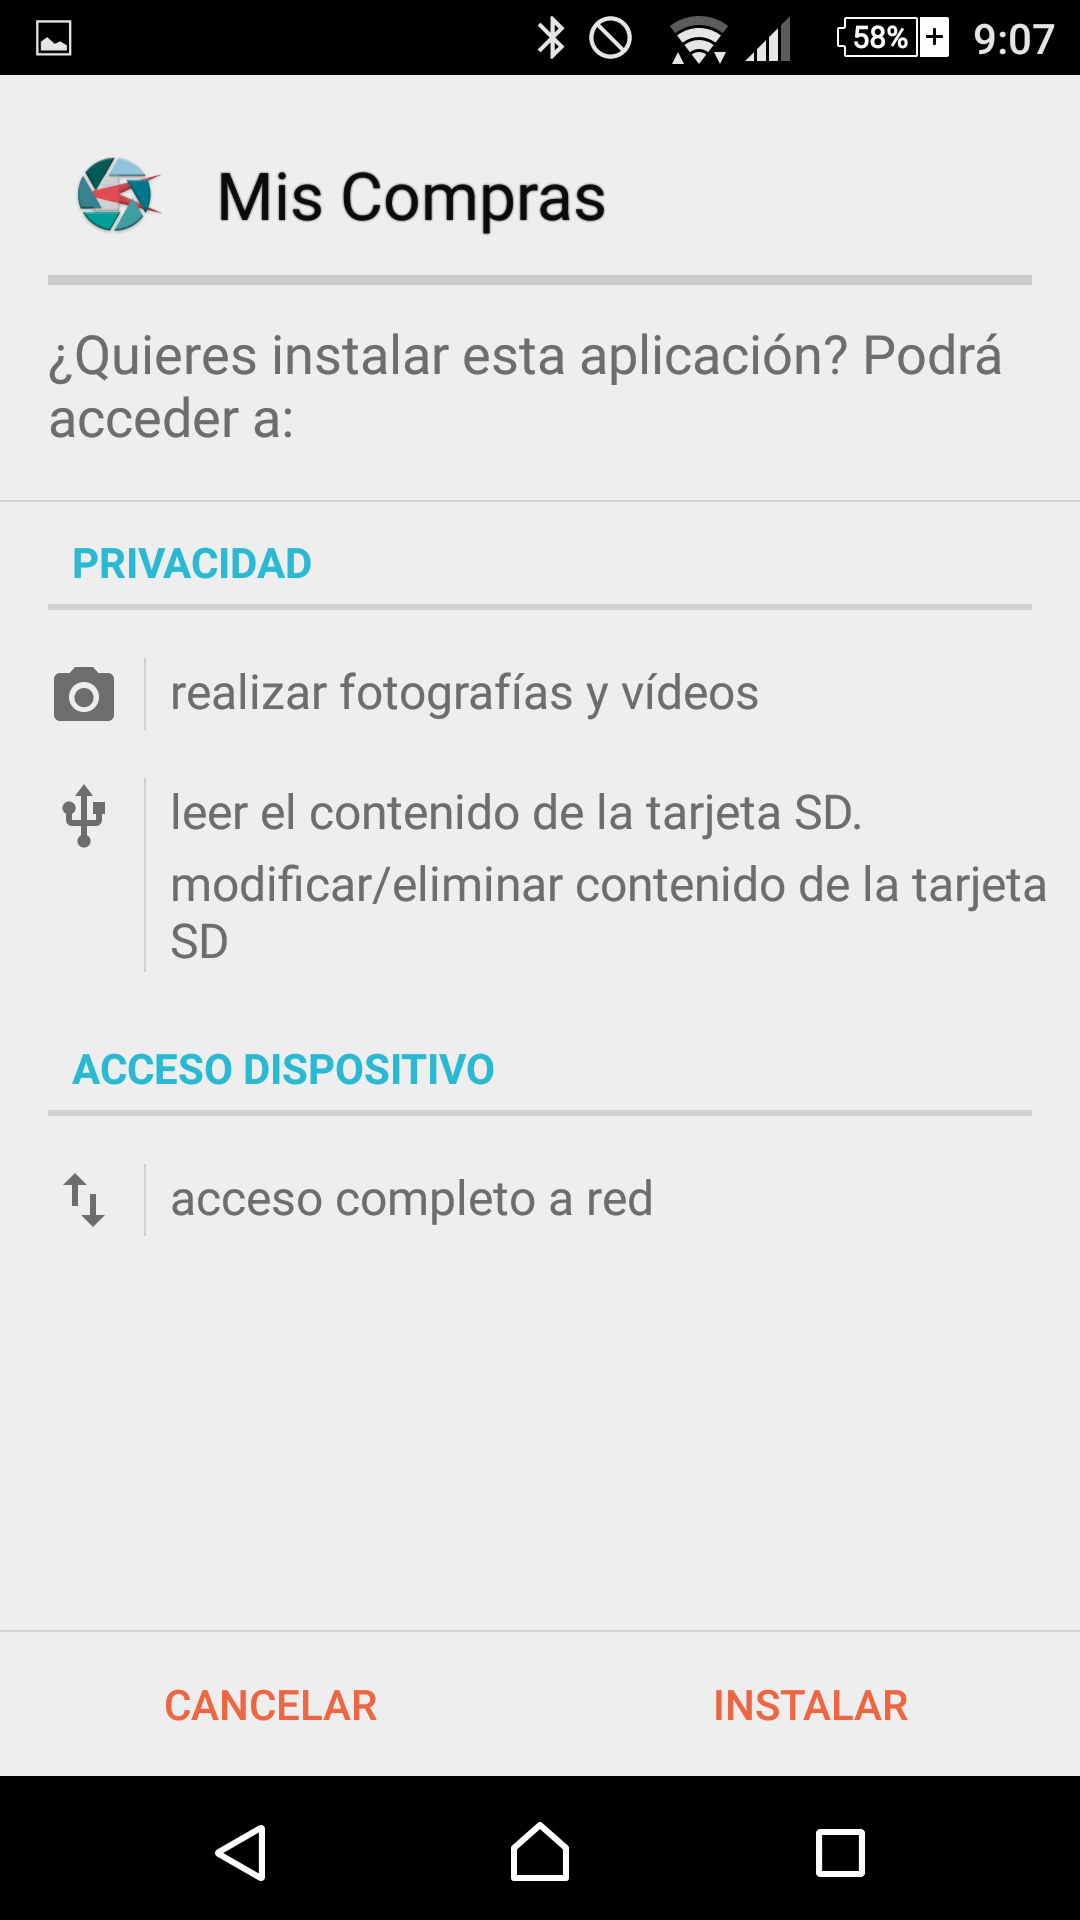
\includegraphics[width=\linewidth]{instalacion1.png}
			\caption{Paso de Instalación 1}
			\label{fig:instalacion1}
	\end{minipage}
	\quad
	\begin{minipage}[b]{0.45\linewidth}
		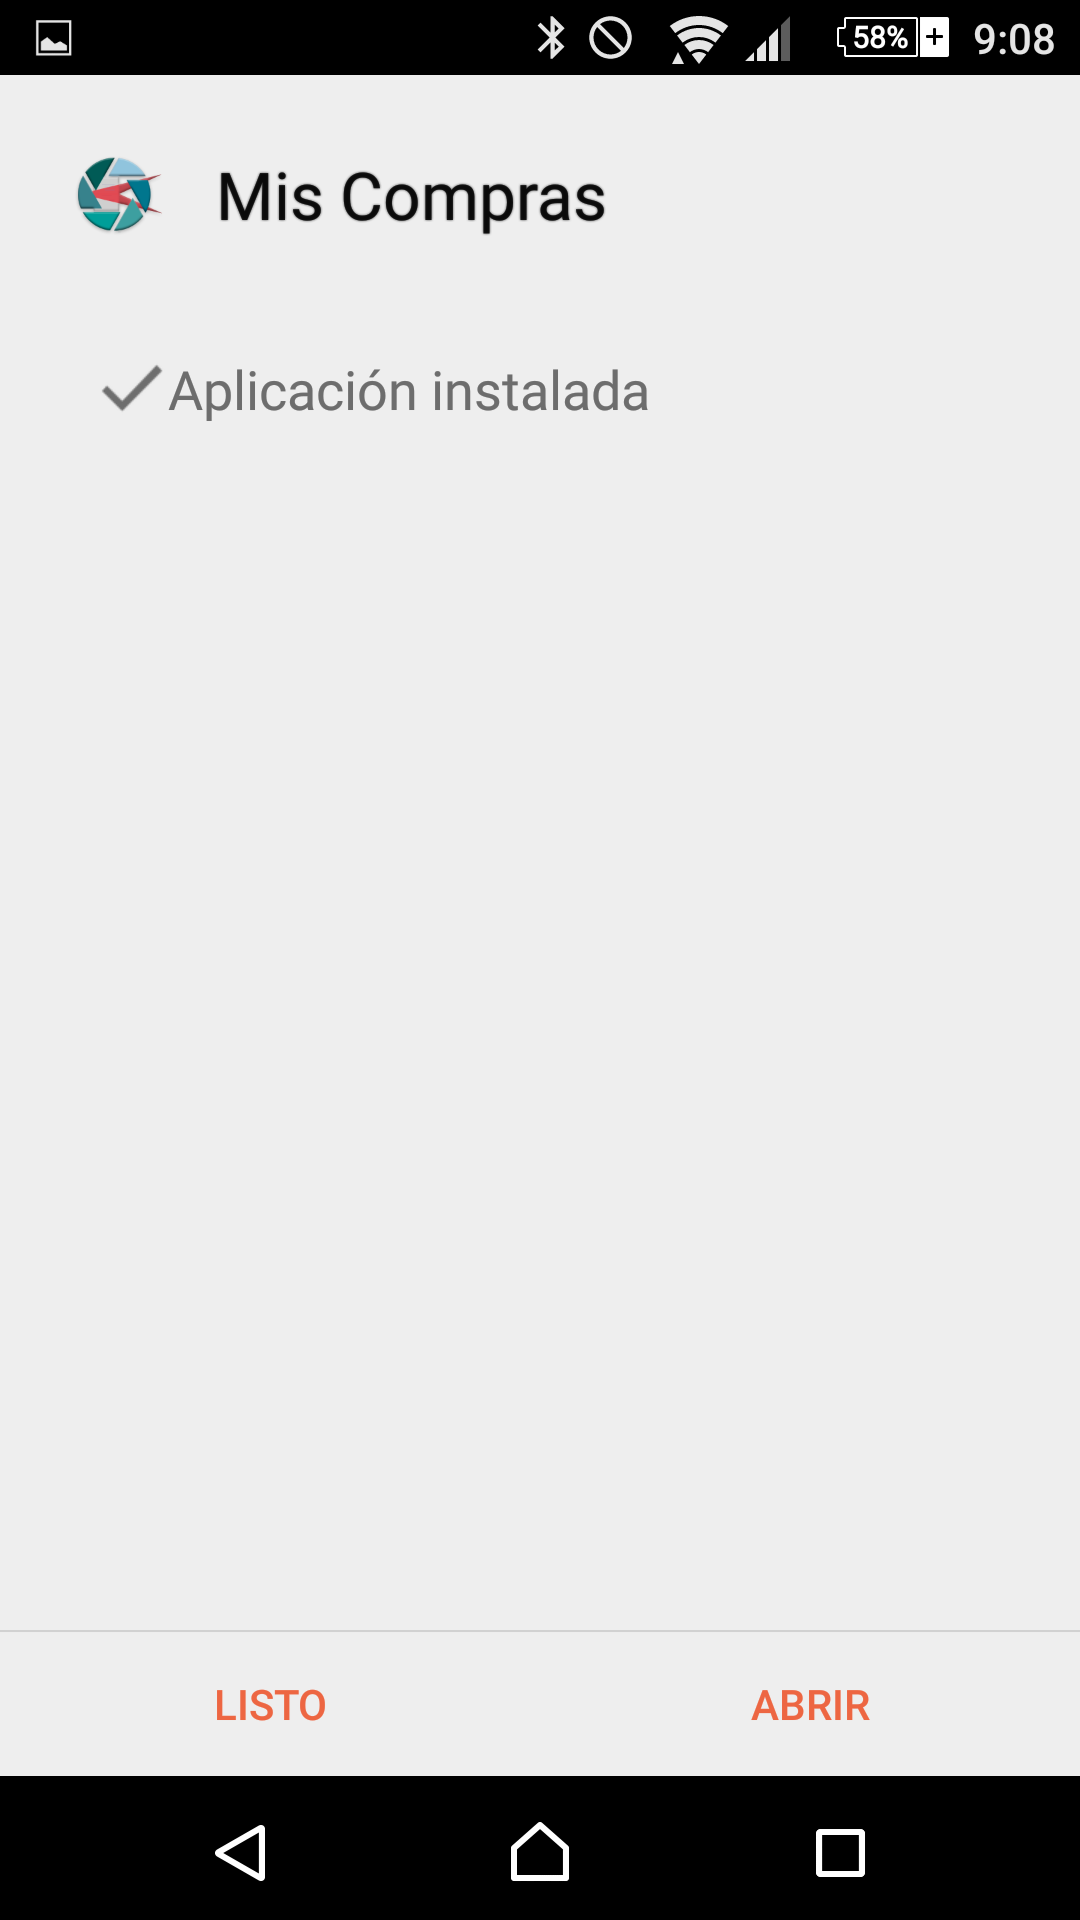
\includegraphics[width=\linewidth]{instalacion2.png}
		\caption{Paso de Instalación 2}
		\label{fig:instalacion2}
		\end{minipage}
	\end{figure}

\cleardoublepage
\section{Manual del usuario}

En esta sección se describe el uso de la aplicación.

\subsection{Menú de opciones de la aplicación. \label{menu}}

El menú de opciones de la aplicación se despliega deslizando el dedo desde el margen izquierdo de la pantalla hacia la derecha.

\begin{figure}[ht]
\begin{center}
\minipage{0.60\textwidth}
  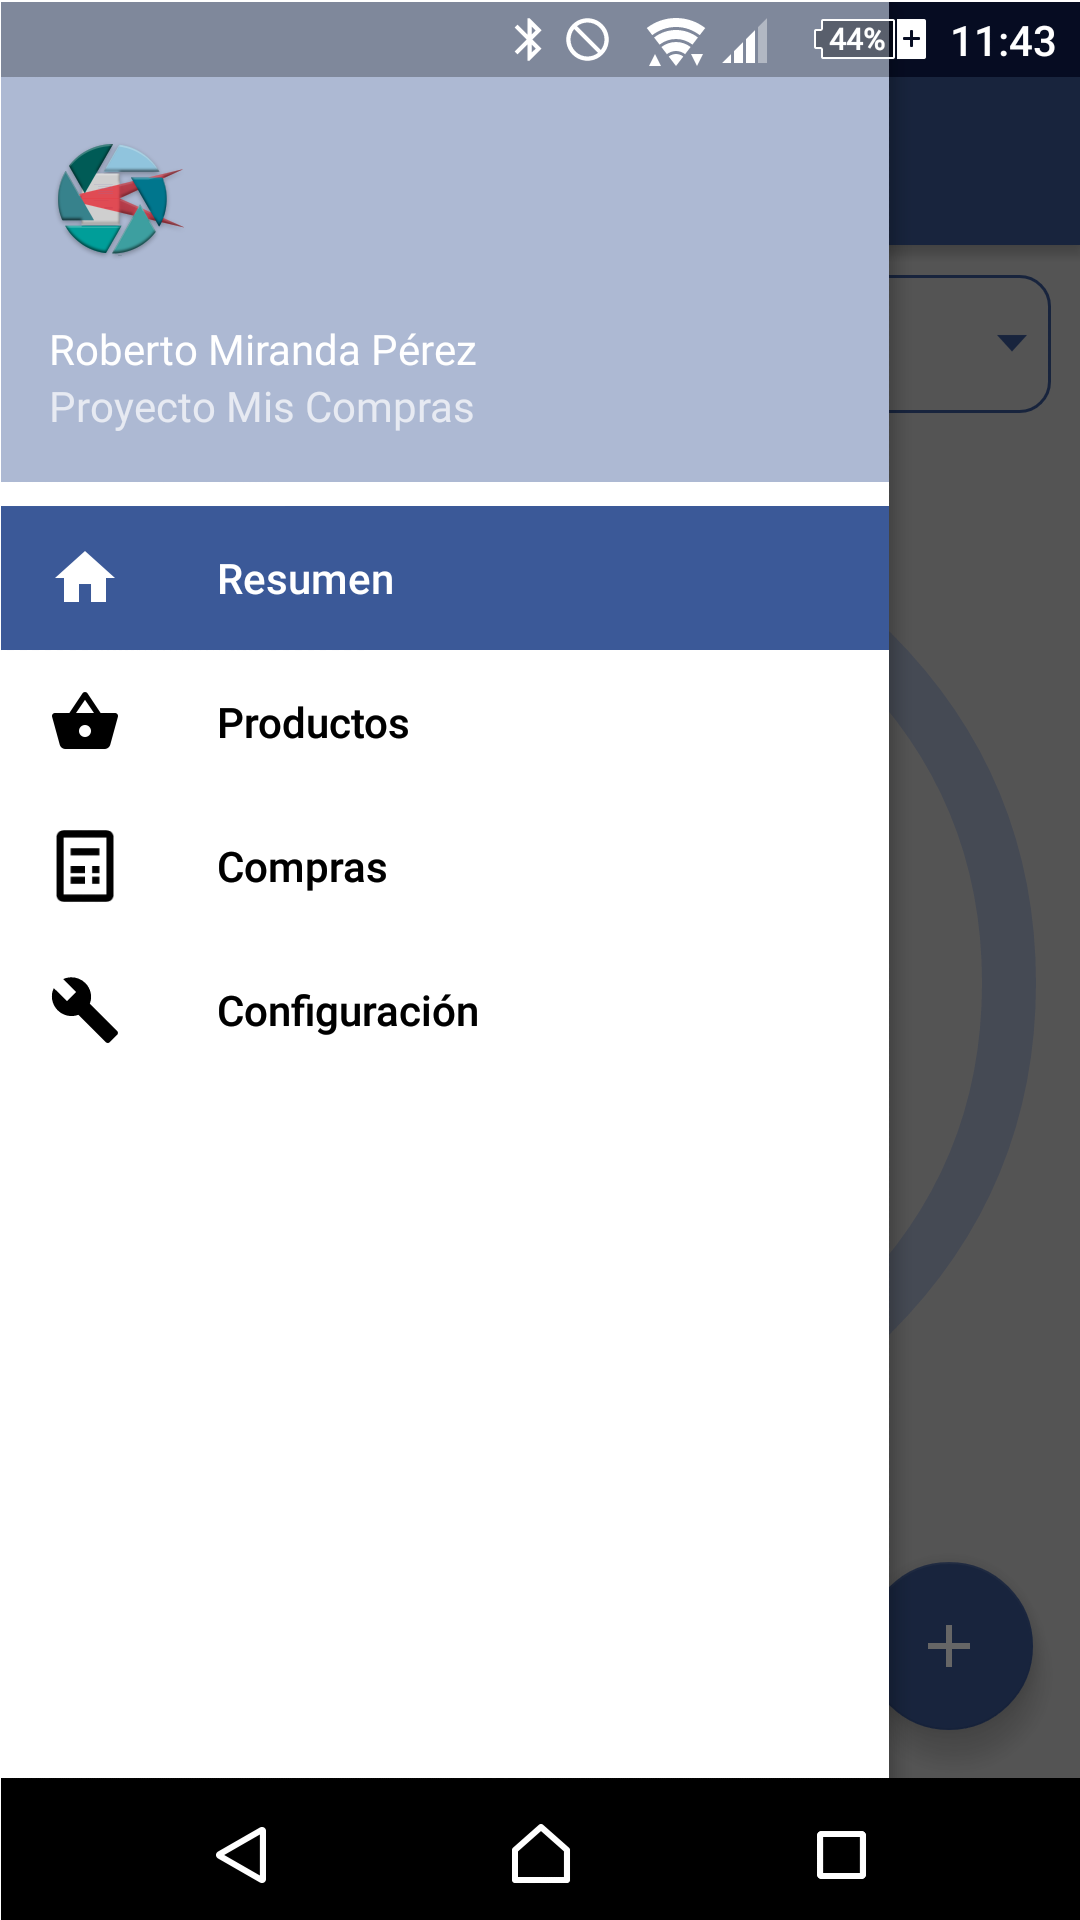
\includegraphics[width=\linewidth]{menu2.png}
  \caption{Menú de la aplicación.}\label{fig:menu}
\endminipage 
\end{center}
\end{figure}

Este menú consta de cuatro opciones que realizan diferentes funciones:
\begin{enumerate}
	\item \textbf{Resumen: }En esta pantalla se muestra un resumen de los gastos del usuario en un gráfico. Se visualiza el importe gastado por categoría y el porcentaje sobre el gasto total. También tiene la opción principal de añadir nuevos tiques (ver sección \ref{resumen} y \ref{nuevosTiques}).
	\item \textbf{Productos: }En esta pantalla se pueden consultar los productos adquiridos, permitiendo cambiar una serie de filtros para su búsqueda(ver sección \ref{consultaProdutos}).
	\item \textbf{Compras: }En esta pantalla se pueden consultar las compras realizadas, permitiendo cambiar una serie de filtros para su búsqueda(ver sección \ref{consultaCompras}).
	\item \textbf{Configuración: } Permite cambiar la dirección ip del servidor. 
\end{enumerate}


\subsection{Añadir Nuevo tique.\label{nuevosTiques}}
 Para empezar a usar la aplicación, pulse en el botón \ref{fig:boton1}
 para añadir una nueva imagen de tique. Este botón permite seleccionar el origen de la imagen que se desea cargar:
 \begin{itemize}
 	\item Botón \ref{fig:boton2} para cargar desde la galería.
 	\item Botón \ref{fig:boton3} para cargar desde la cámara.
 \end{itemize}
 \begin{figure}[!htb] 
\minipage{0.32\textwidth}
  
\includegraphics[width=\linewidth]{boton1.png}
  \caption{Añadir nueva imagen}\label{fig:boton1}
\endminipage\hfill
\minipage{0.32\textwidth}
  
\includegraphics[width=\linewidth]{boton2.png}
  \caption{Imagen de galeria}\label{fig:boton2}
\endminipage\hfill
\minipage{0.32\textwidth}%
  
\includegraphics[width=\linewidth]{boton3.png}
  \caption{Imagen de camara}\label{fig:boton3}
\endminipage
\end{figure}

Una ver seleccionada la imagen, seleccione el área del tique donde se encuentran los productos adquiridos utilizando el cuadro que se muestra encima de la imagen (ver figura \ref{fig:cargaImagen} , y pulse \textbf{Recortar} para empezar el proceso. Si desea cargar una imagen distinta, pulse en el botón \textbf{Cancelar}. 
\begin{figure}[ht]
\begin{center}
\minipage{0.60\textwidth}
  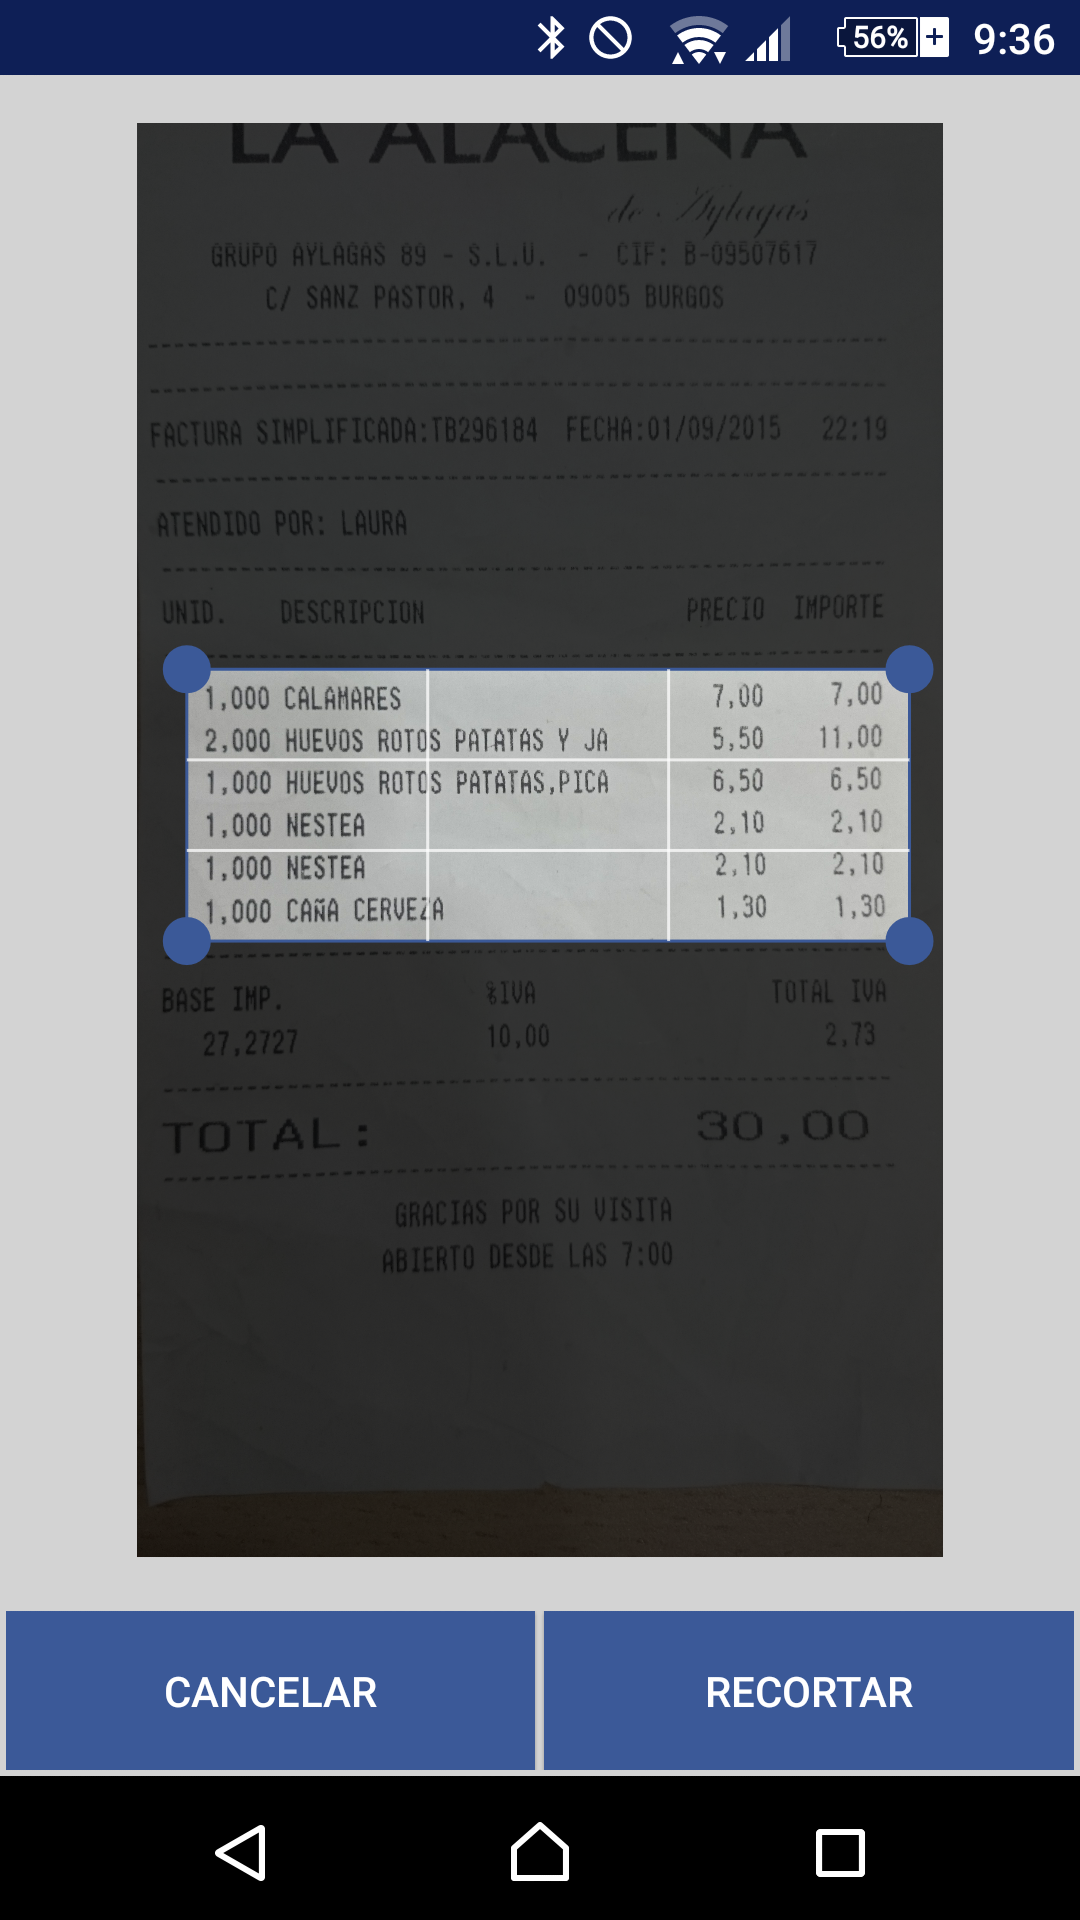
\includegraphics[width=\linewidth]{cargaImagen.png}
  \caption{Proceso de carga de nuevo tique.}\label{fig:cargaImagen}
\endminipage 
\end{center}
\end{figure}

Cuando empieza el proceso de carga de la imagen, se muestra un diálogo de progreso(ver figura \ref{fig:subida}), que una vez terminado si la imagen se ha procesado correctamente permitirá editar los elementos, sin embargo si hay algún error durante el proceso o conversión de la imagen, se mostrara un mensaje de error en la pantalla.
\imagen{subida}{Diálogo de subida}

Completado este proceso, se visualiza en formato de lista los elementos obtenidos(ver figura \ref{fig:cargaProductos}), si hay algún error de conversión el importe del producto se muestra en rojo, por el contrario si todo ha ido bien el color será verde.
En la cabecera del tique se detalla la fecha y el importe total de la compra.

Para poder editar un producto (cantidad, nombre, precio y categoría), se debe pulsar sobre el elemento que se quiere modificar, que abrirá un diálogo de edición. En este, se deben colocar los nuevos valores que se quieren para el producto(ver figura \ref{fig:dialogoEdicion}).

\begin{figure}[ht]
\minipage{0.45\textwidth}
  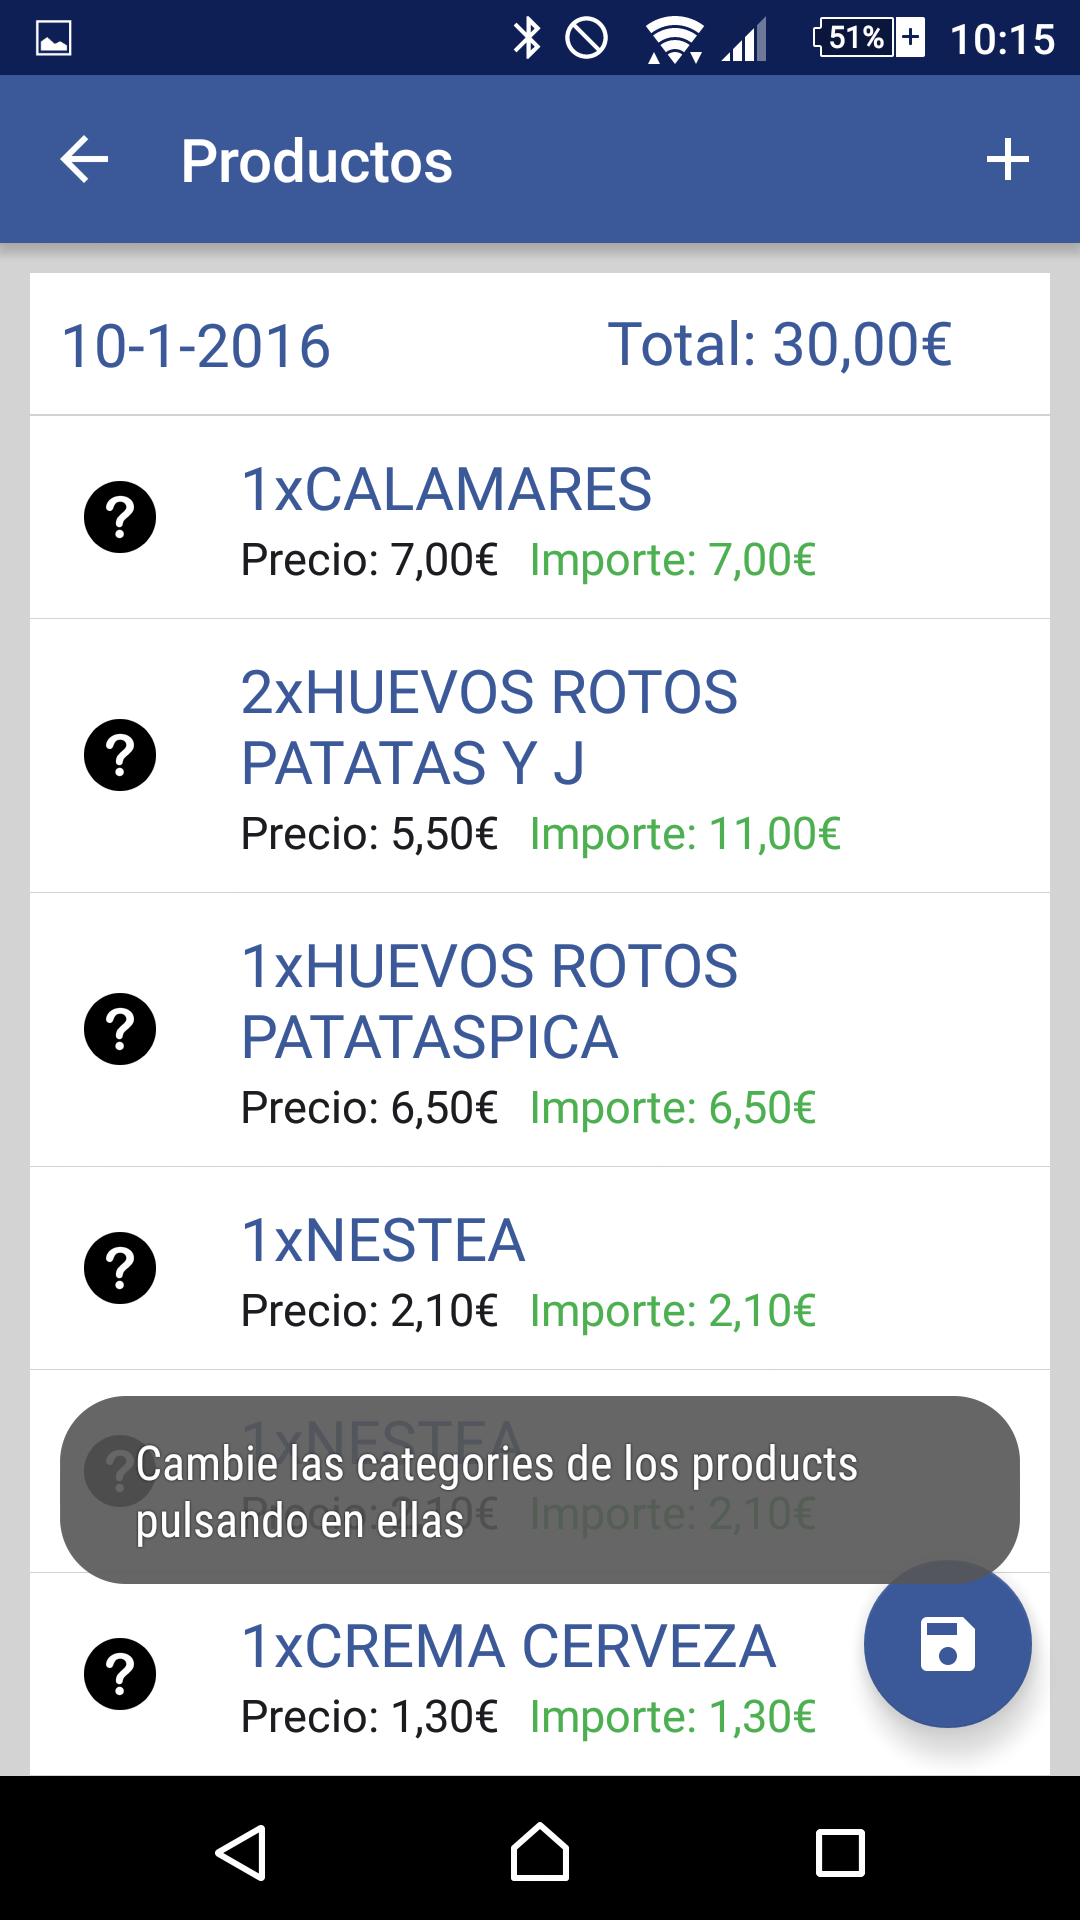
\includegraphics[width=\linewidth]{cargaProductos.png}
  \caption{Carga de nuevos productos.}\label{fig:cargaProductos}
\endminipage\hfill
\minipage{0.45\textwidth}
  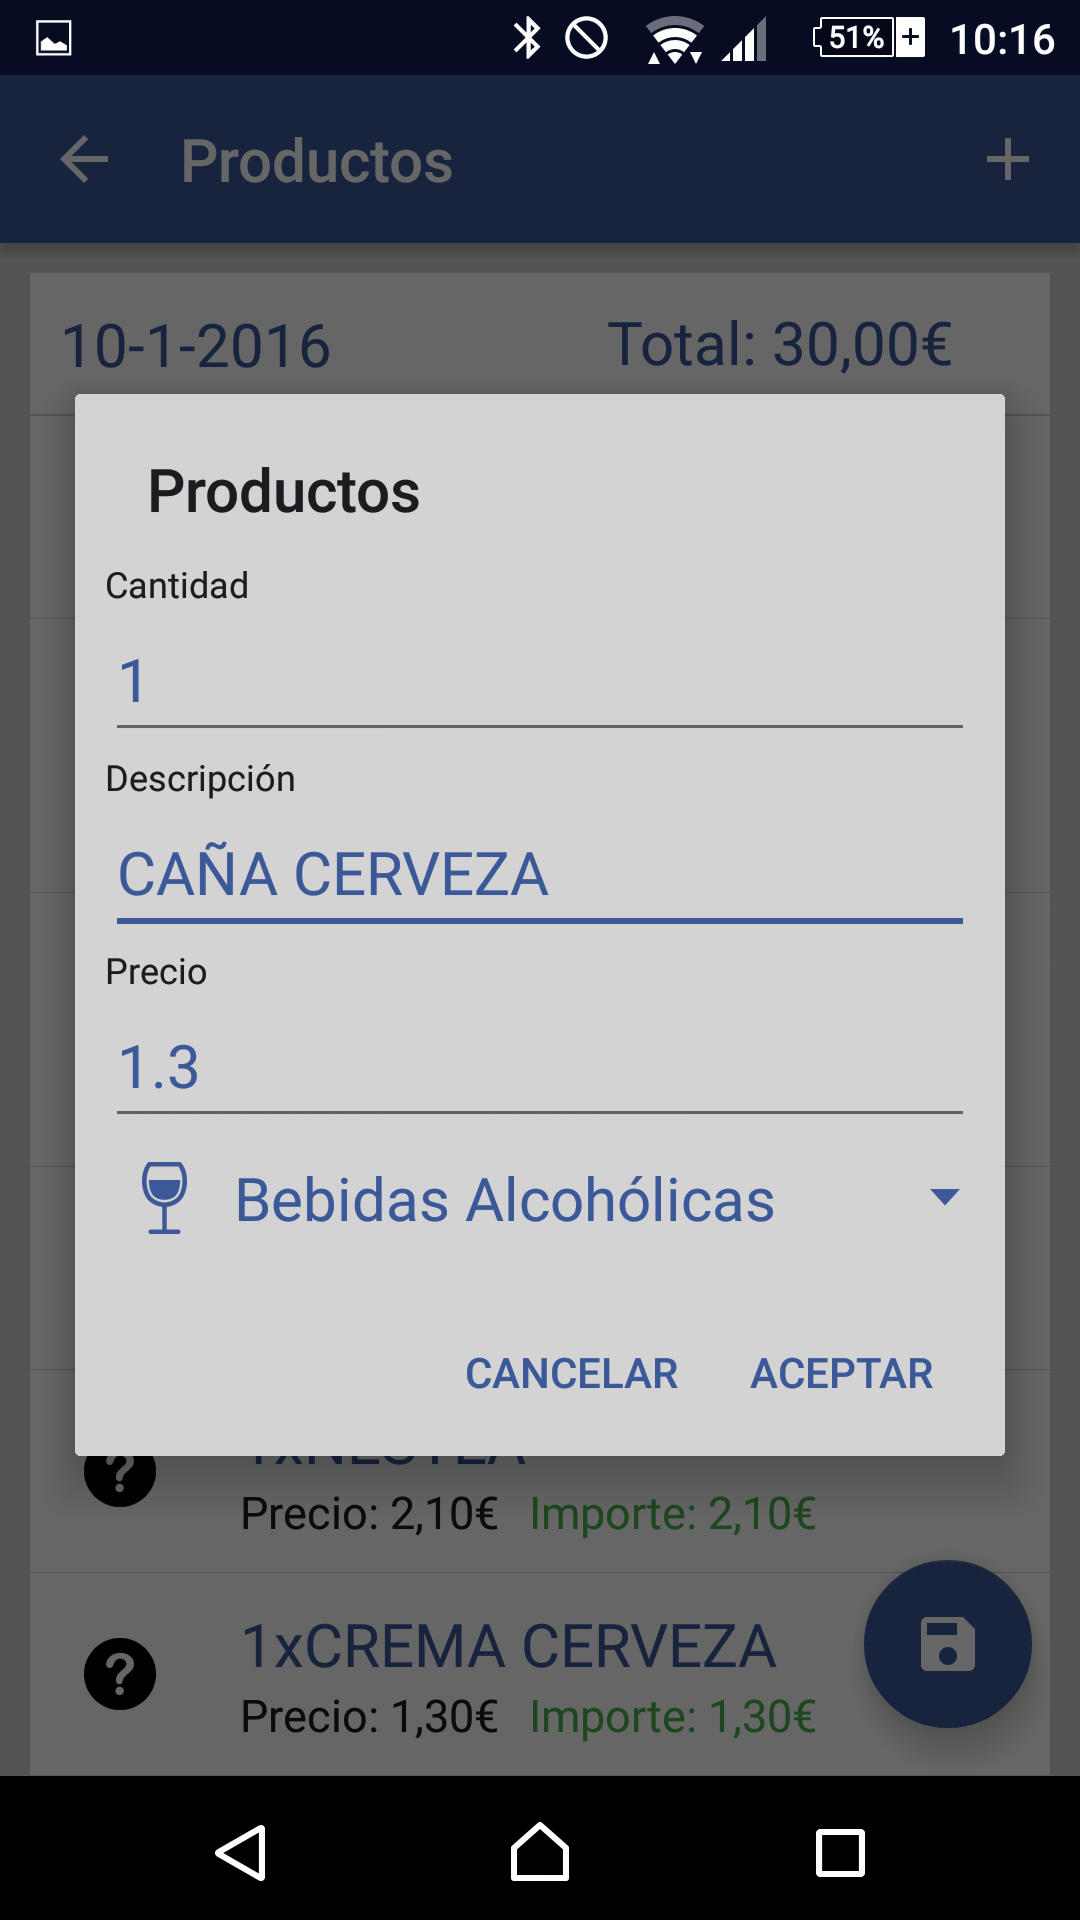
\includegraphics[width=\linewidth]{dialogoEdicion.png}
  \caption{Edición de un producto.}\label{fig:dialogoEdicion}
\endminipage
\end{figure}
\begin{figure}[ht]
\begin{center}
\minipage{0.60\textwidth}%
  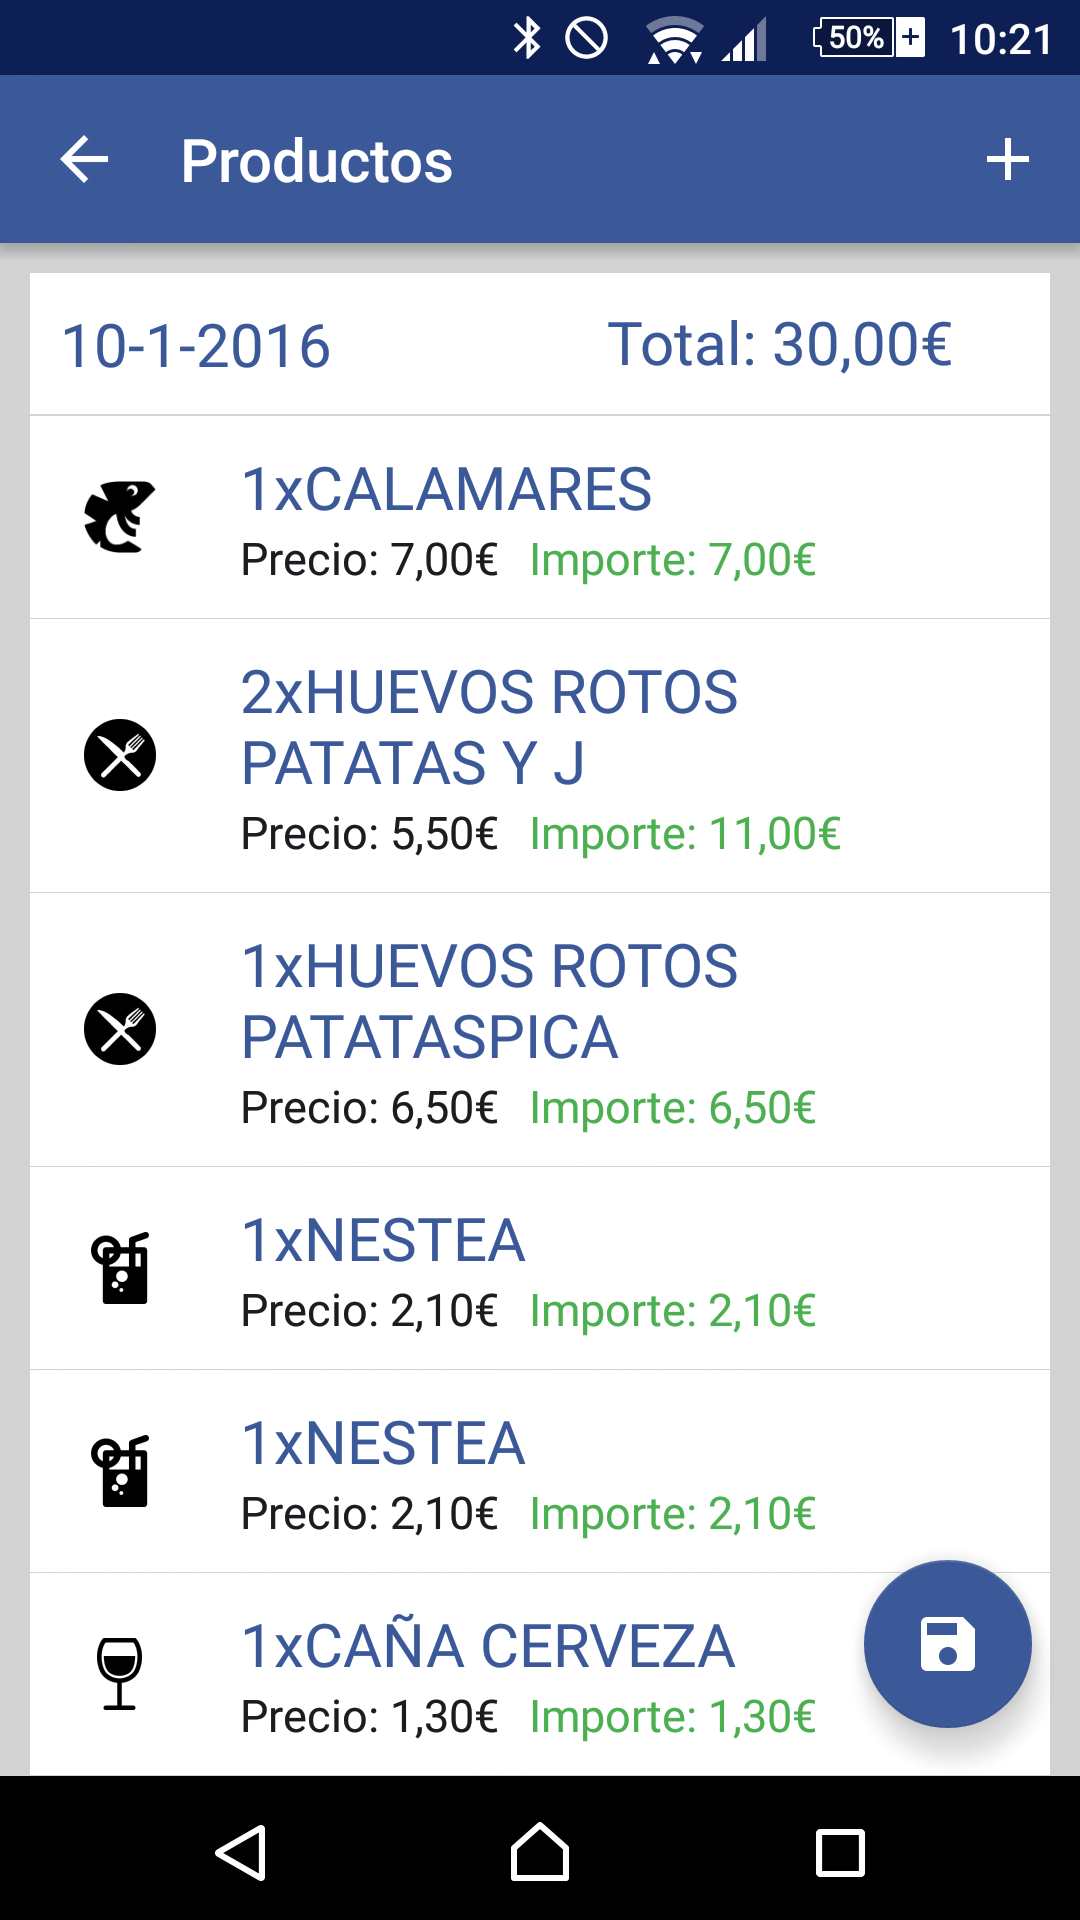
\includegraphics[width=\linewidth]{cargaCompleta.png}
  \caption{Proceso completado.}\label{fig:cargaCompleta}
\endminipage
\end{center} 
\end{figure}
\cleardoublepage
Cuando todos los productos sean correctos, pulsar en el botón \ref{fig:botonGuardar} para guardar, por el contrario si se desea añadir nuevos productos, hay que pulsar el botón \ref{fig:botonAnadir} situado en la esquina superior derecha, que se mostrará un diálogo similar al de edición(ver figura\ref{fig:dialogoEdicion}) para añadir un nuevo producto a la lista.

\begin{figure}[ht]
\begin{center} 
\minipage{0.32\textwidth}
  
\includegraphics[width=\linewidth]{botonGuardar.png}
  \caption{Guardar productos.}\label{fig:botonGuardar}
\endminipage\hfil
\minipage{0.32\textwidth}
  
\includegraphics[width=\linewidth]{botonAnadir.png}
  \caption{Añadir nuevo producto.}\label{fig:botonAnadir}
\endminipage
\end{center}
\end{figure}

\subsection{Vista de Resumen \label{resumen}}

Para ver el resumen de gastos se tiene  que pulsar la opción \textbf{Resumen} del menú de la aplicación(ver sección \ref{menu}).

En el gráfico se puede ver el gasto por categoría y el porcentaje sobre el gasto total que lleva el usuario acumulado.

\begin{figure}[ht]
\begin{center}
\minipage{0.60\textwidth}
  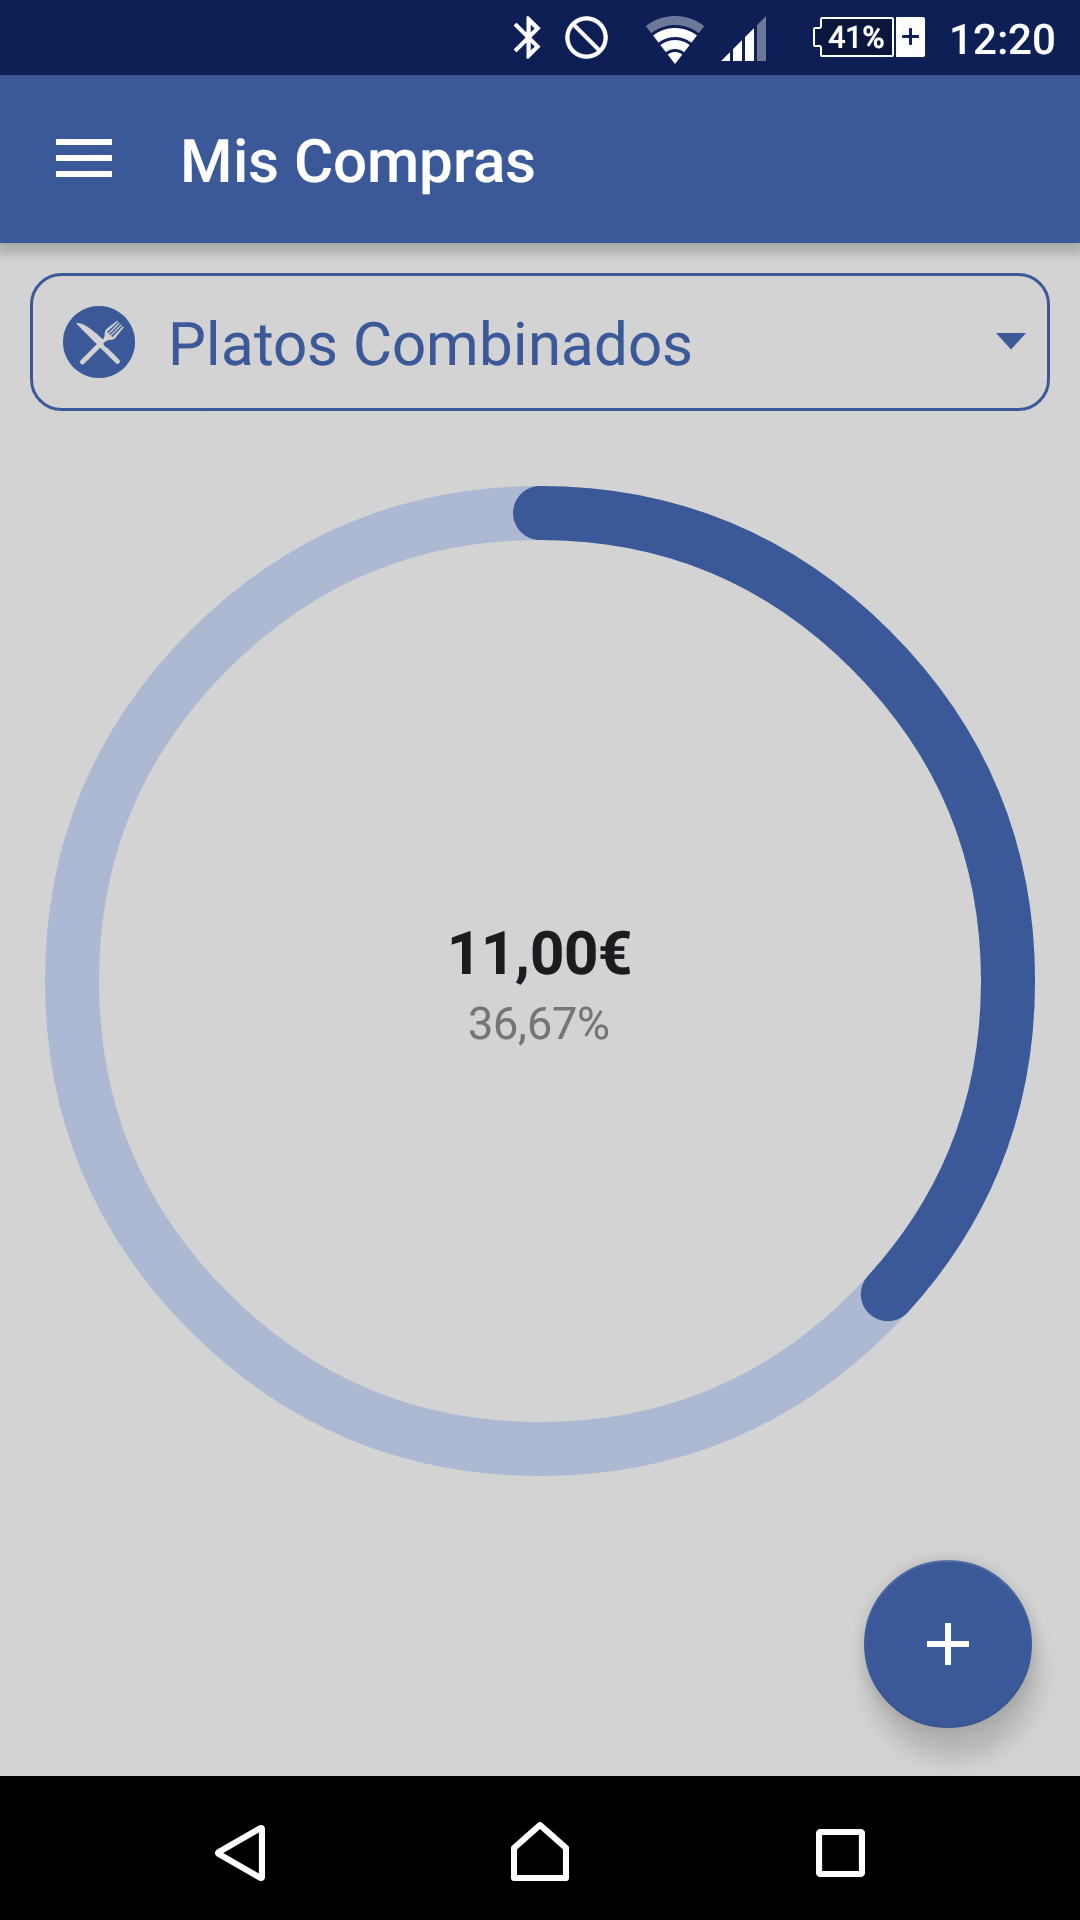
\includegraphics[width=\linewidth]{resumen.png}
  \caption{Vista de Resumen.}\label{fig:resumen}
\endminipage 
\end{center}
\end{figure} 

\cleardoublepage
\subsection{Consulta de Productos \label{consultaProdutos}}

Para consultar los productos adquiridos se tiene que pulsar la opción \textbf{Productos} del menú de la aplicación(ver sección \ref{menu}).

En la pantalla de Productos para realizar una consulta basta con pulsar el botón con el icono de lupa(ver figura \ref{fig:botonBusqueda}). 

\begin{figure}[ht]
\begin{center}
\minipage{0.32\textwidth}
  
\includegraphics[width=\linewidth]{botonBusqueda.png}
  \caption{Botón  de bisqueda.}\label{fig:botonBusqueda}
\endminipage
\end{center}
\end{figure}

Para realizar diferentes consultas se puede cambiar entre varias opciones, para poder cambiar los filtros de búsqueda se tiene que pulsar el botón de menú, situado en la esquina superior derecha de la pantalla y seleccionar la opción de filtros.

\imagen{opcionFiltros}{Filtro de productos.}

Cuando se pulsa en este botón, aparece un diálogo de selección del filtro deseado(ver figura \ref{fig:filtrosProducto} ), siendo estos \textbf{Fechas, Precio Unitario, Categoría}
\begin{itemize}
	\item \textbf{Fecha: }Fecha de compra del producto.
	\item\textbf{Precio Unitario: }Precio del producto.
	\item \textbf{Categoría: } Categoría del producto.
\end{itemize} Cuando se seleccione otro filtro, este cambia en la pantalla principal (ver figuras \ref{fig:filtroFechas}, \ref{fig:filtroPrecios} y \ref{fig:filtroCategorias}).



\begin{figure}[ht]
\begin{center}
\minipage{0.45\textwidth}
  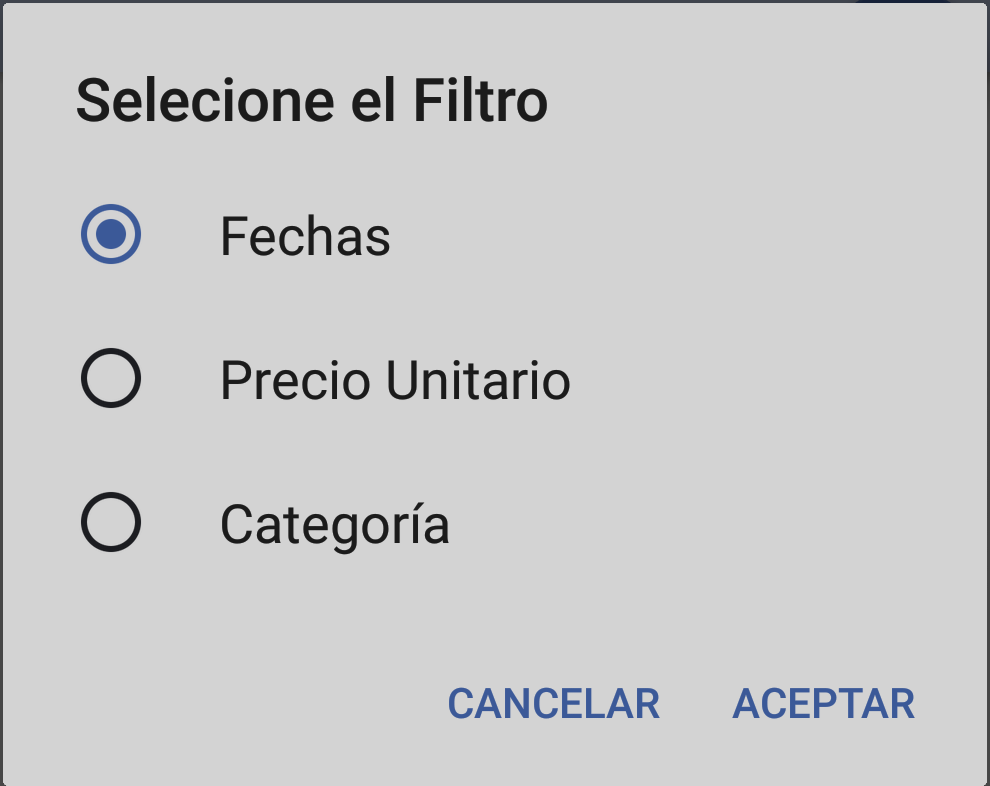
\includegraphics[width=\linewidth]{filtrosProducto.png}
  \caption{Filtros de busqueda de productos}\label{fig:filtrosProducto}
\endminipage
\end{center}
\end{figure}

\begin{figure}[ht]
\begin{center}
\minipage{0.60\textwidth}
  
\includegraphics[width=\linewidth]{filtroFechas.png}
  \caption{Filtro por fechas.}\label{fig:filtroFechas}
\endminipage 
\end{center}
\end{figure}

\begin{figure}[ht]
\begin{center}
\minipage{0.60\textwidth}
  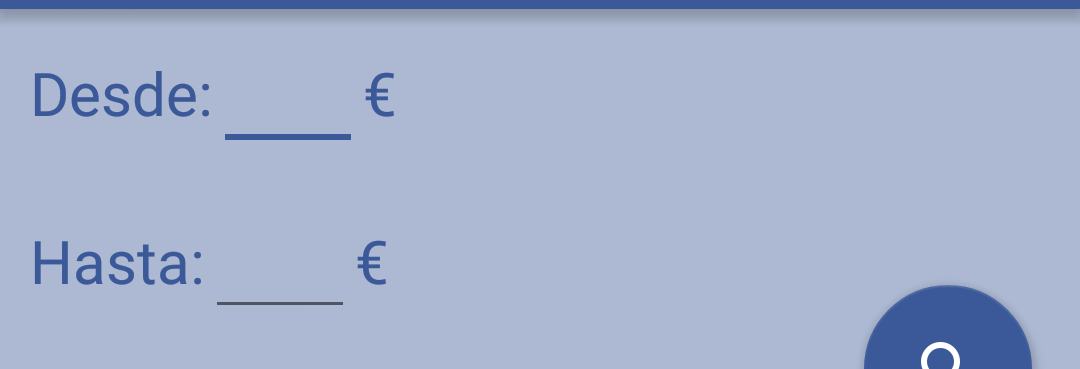
\includegraphics[width=\linewidth]{filtroPrecios.png}
  \caption{Filtro por precios.}\label{fig:filtroPrecios}
\endminipage 
\end{center}
\end{figure}

\begin{figure}[ht]
\begin{center}
\minipage{0.60\textwidth}
  \includegraphics[width=\linewidth]{filtroCategorias.png}
  \caption{Filtro por categorías.}\label{fig:filtroCategorias}
\endminipage 
\end{center}
\end{figure}
\cleardoublepage
Una vez seleccionado el filtro deseado y rellenado correctamente, al pulsar el botón de búsqueda(ver figura \ref{fig:botonBusqueda}) se muestra una lista de productos que cumplen el filtro seleccionado.

\begin{figure}[ht]
\begin{center}
\minipage{0.60\textwidth}
  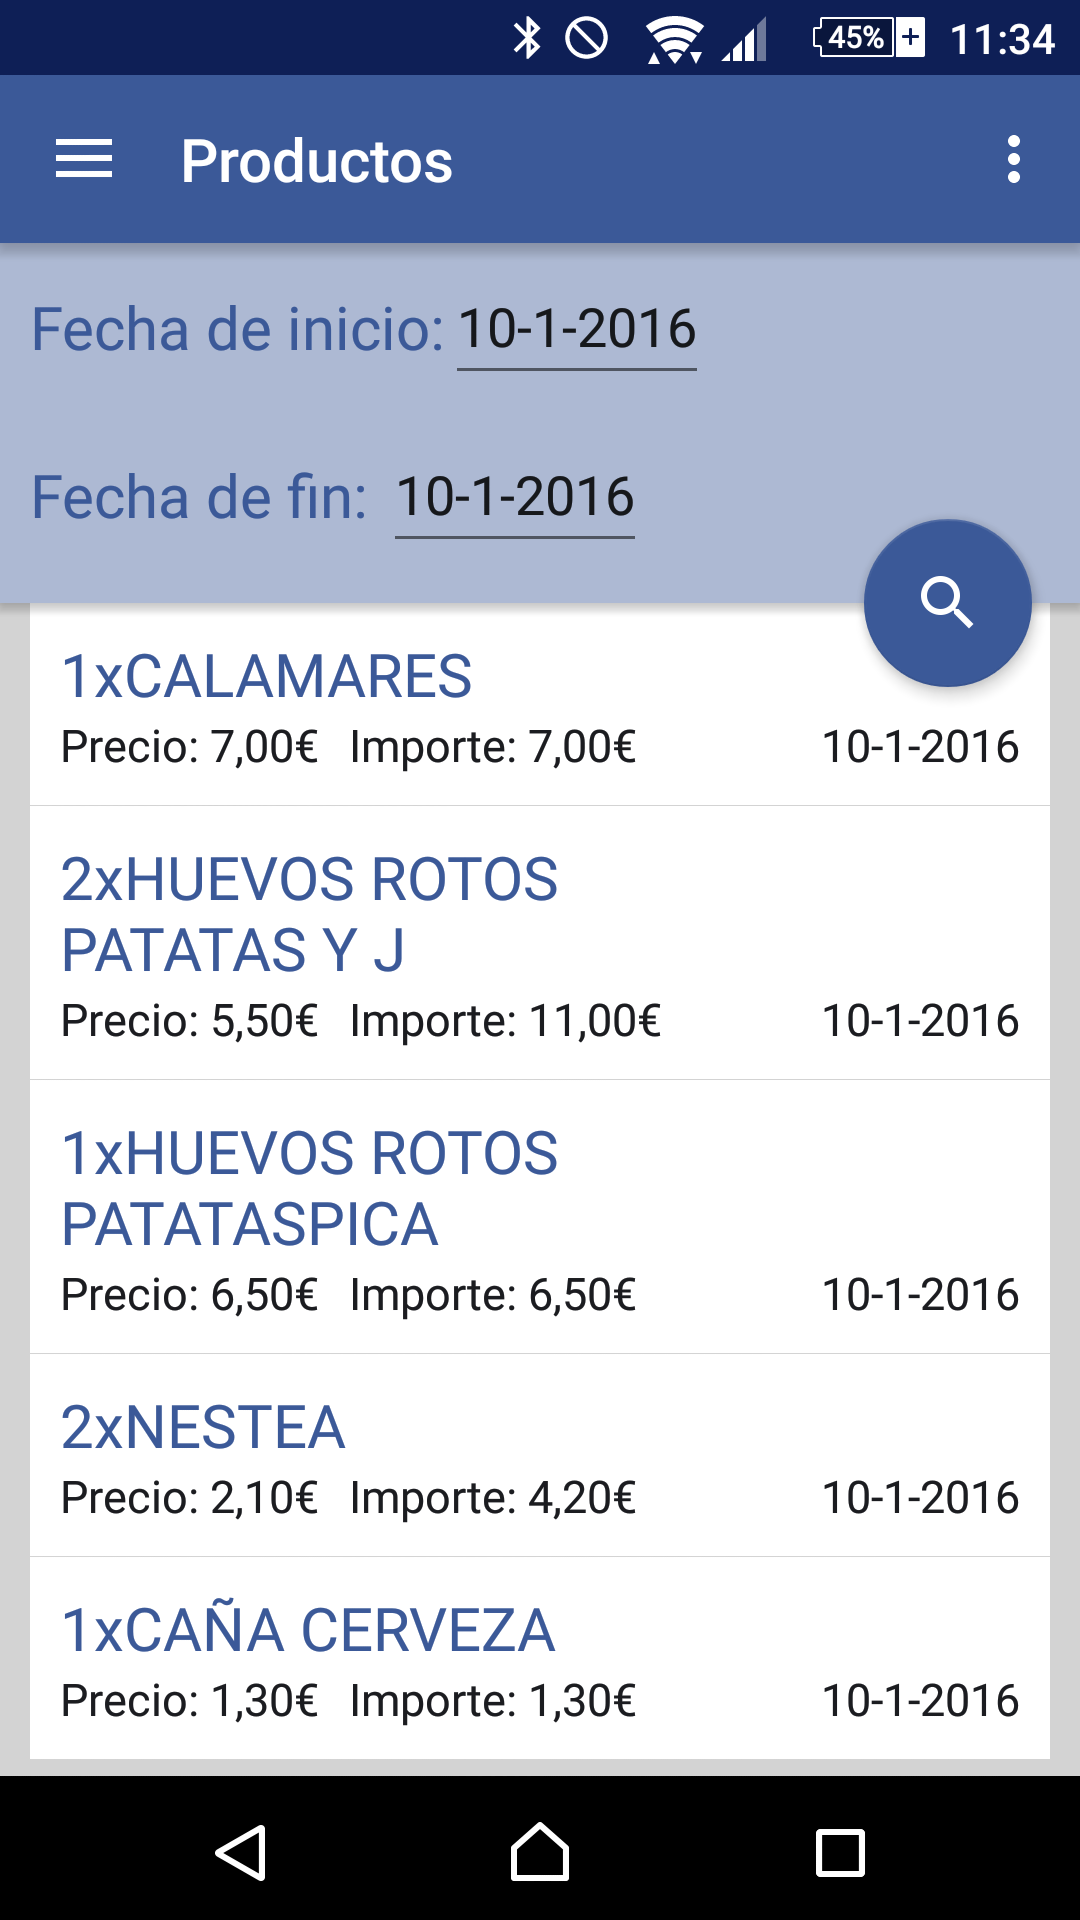
\includegraphics[width=\linewidth]{listaProductos.png}
  \caption{Ejemplo de lista de productos.}\label{fig:listaProductos}
\endminipage 
\end{center}
\end{figure}

\cleardoublepage

\subsection{Consulta de Compras \label{consultaCompras}} 

Para consultar las compras se tiene que pulsar la opción \textbf{Compras} del menú de la aplicación(ver sección \ref{menu}).

El proceso de consulta de compras es igual que en la consulta de productos(ver sección\ref{consultaProdutos}). Al terminar de realizar las consultas se obtiene una lista con las compras que cumplan los requisitos del filtro.
\begin{figure}[ht]
\begin{center}
\minipage{0.60\textwidth}
  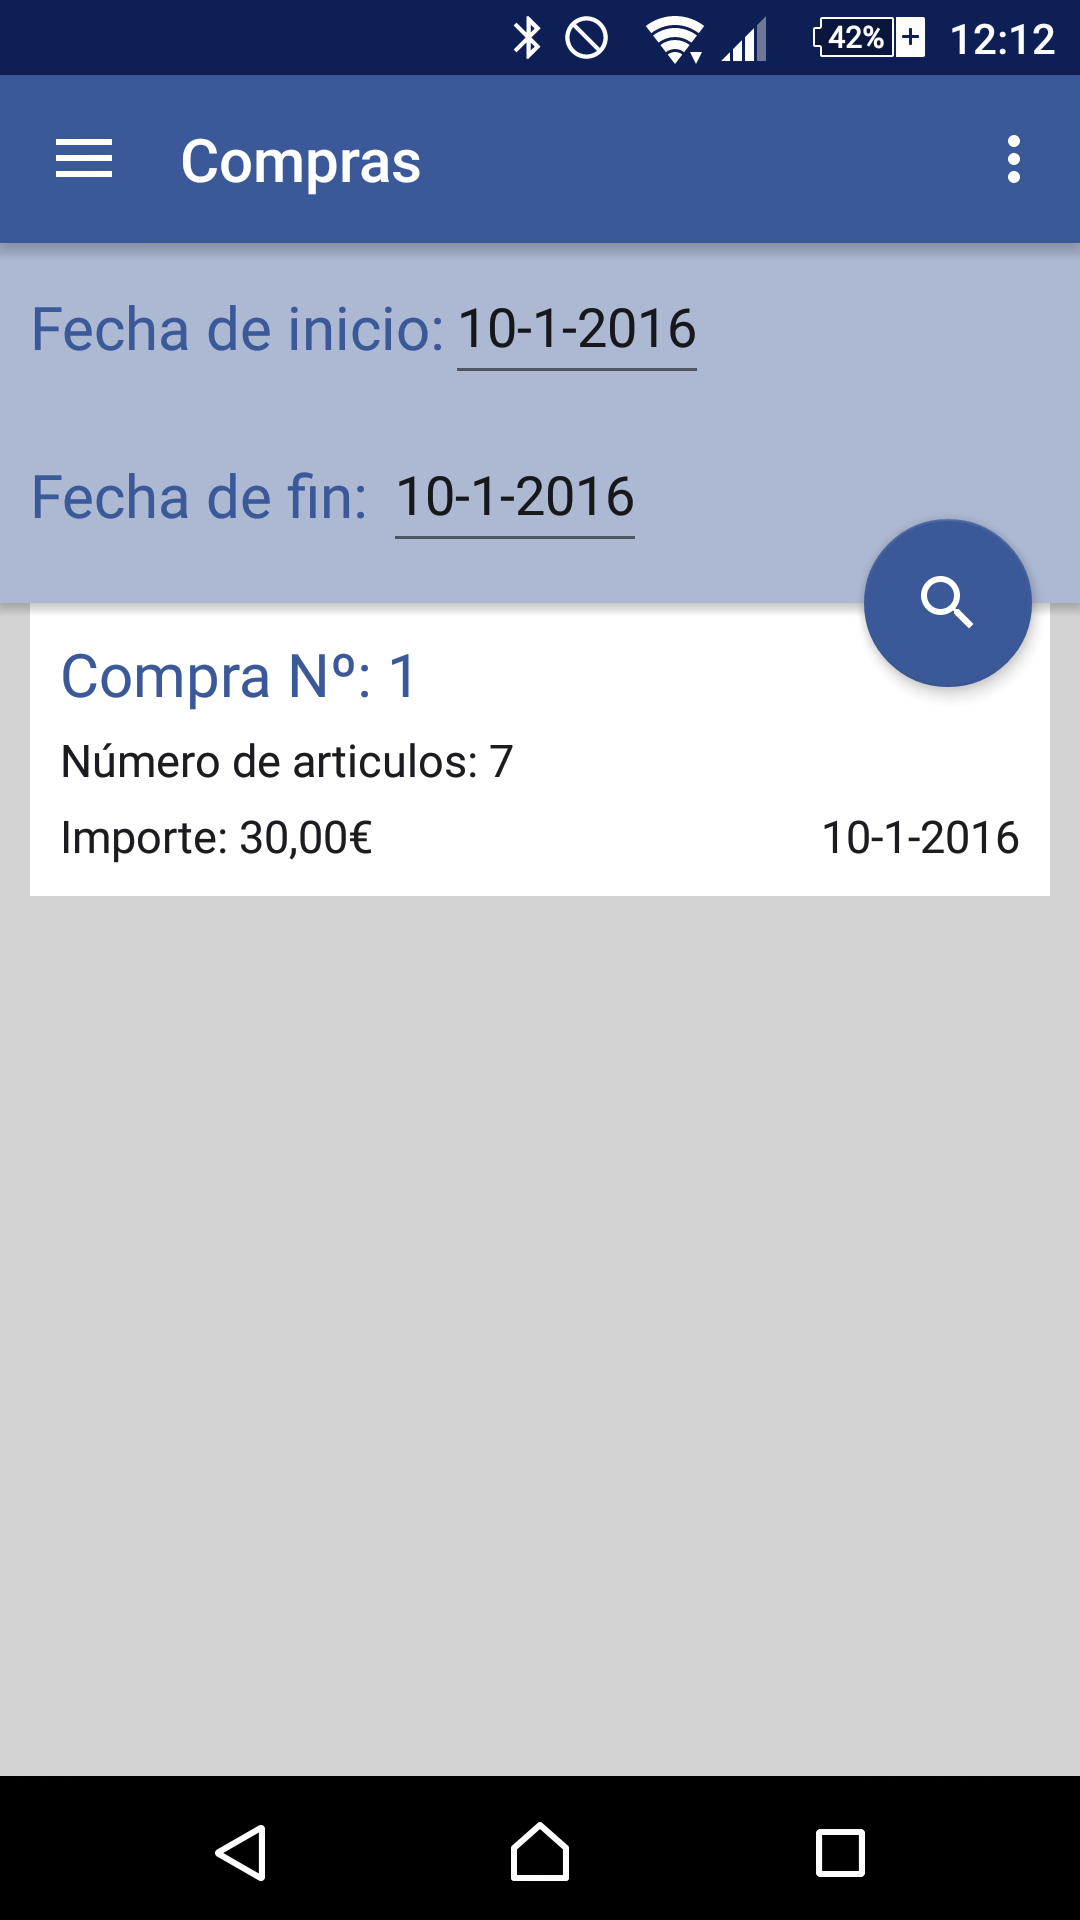
\includegraphics[width=\linewidth]{listaCompras.png}
  \caption{Ejemplo lista de compras.}\label{fig:listaCompras}
\endminipage 
\end{center}
\end{figure}

En este caso los filtros son:
\begin{itemize}
	\item \textbf{Fecha: }Fecha de compra.
	\item\textbf{Importe: }Importe de la compra.
\end{itemize}

Si se pulsa sobre un elemento de la lista, se cambia a una vista de detalle de los productos adquiridos en la compra seleccionada compra(ver figura \ref{fig:detalleTique}).

\begin{figure}[ht]
\begin{center}
\minipage{0.60\textwidth}
  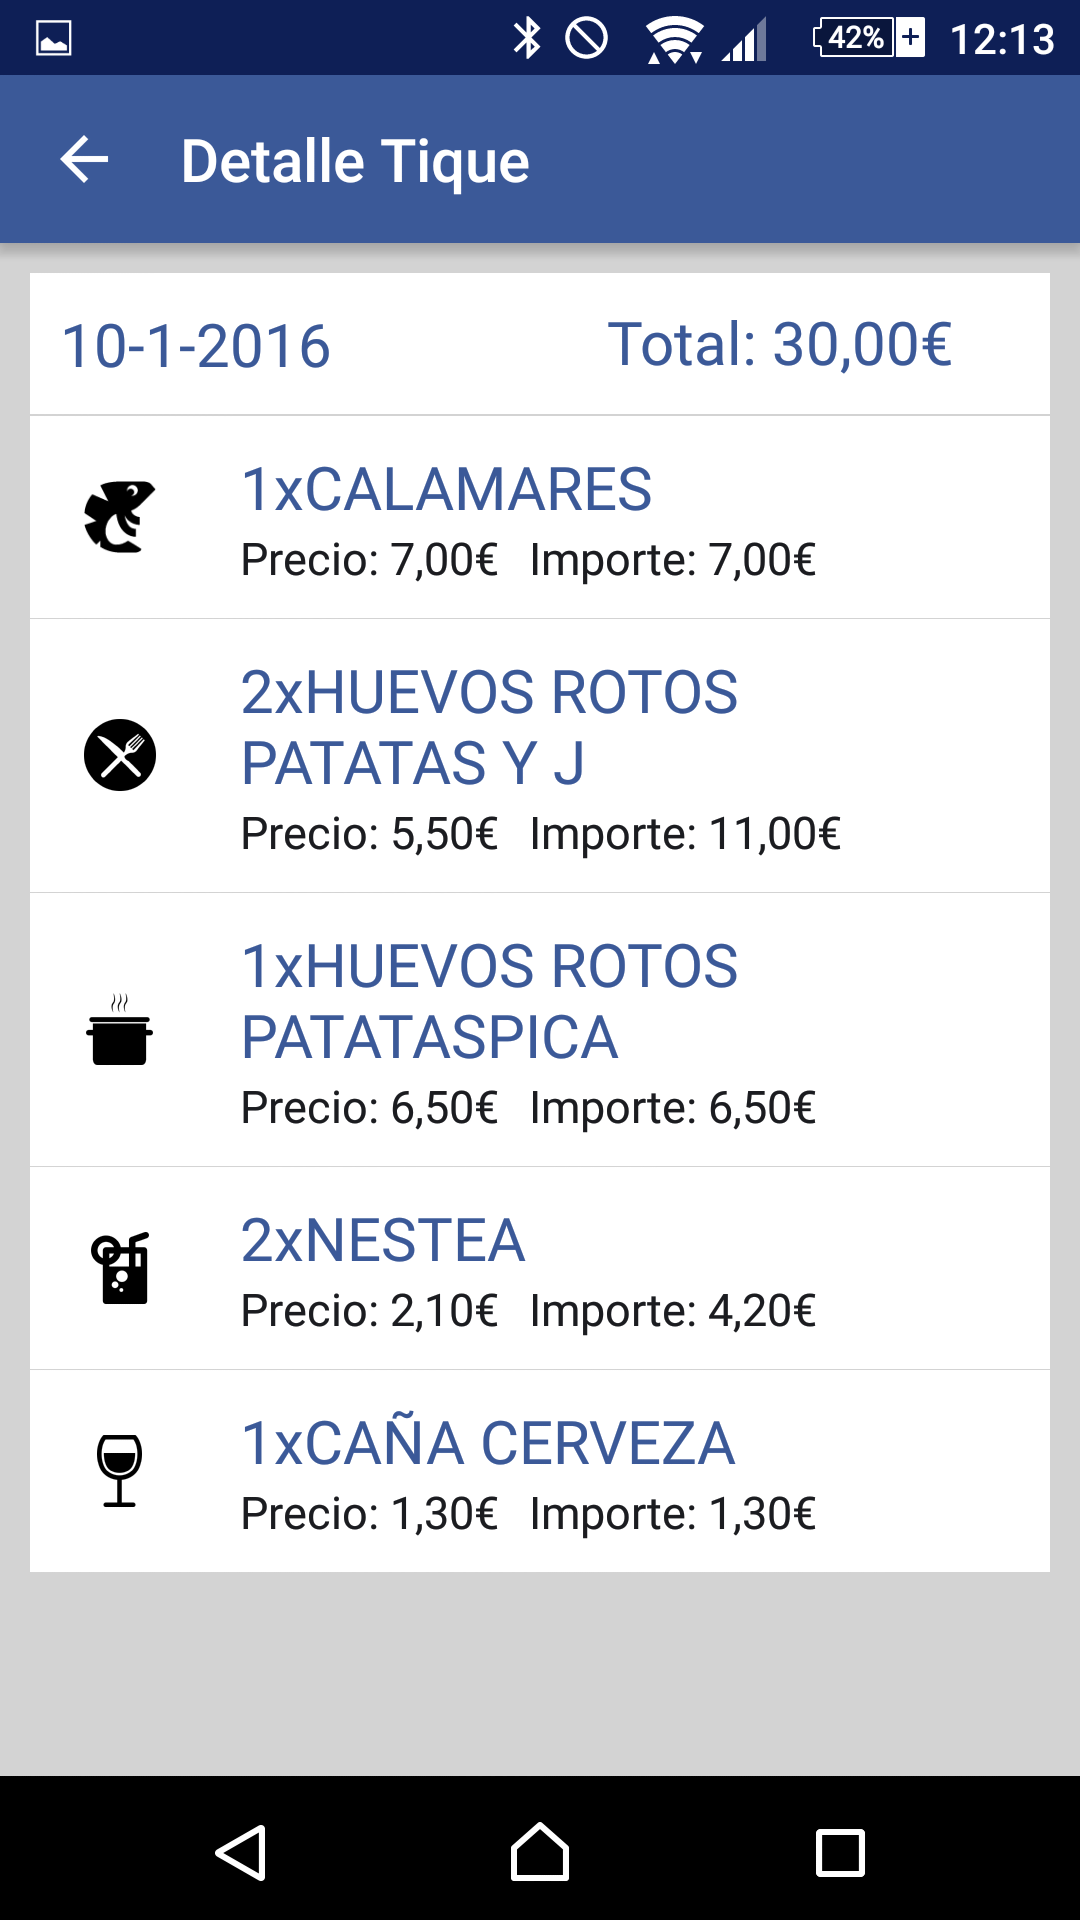
\includegraphics[width=\linewidth]{detalleTique.png}
  \caption{Vista de detalle de una compra.}\label{fig:detalleTique}
\endminipage 
\end{center}
\end{figure}


\bibliographystyle{plain}
\bibliography{bibliografiaAnexos}

\end{document}